\documentclass[11pt]{beamer}
\usetheme{Warsaw}
\usepackage[spanish]{babel}     % for proper word breaking at line ends
\usepackage[utf8]{inputenc}
\usepackage[T1]{fontenc}
\usepackage{amsmath}
\usepackage{amsfonts}
\usepackage{amssymb}
\usepackage{graphicx}
\usepackage{subfig}
\usepackage[export]{adjustbox}
%%%%%%%%%%%%%%%%%%%%%%%%%%%%%%%%%%%%%%%%%%%%%%%%%%%%%%%%%%%%%%%%%%%%%%%%%%%%%%%%%5
\author{Fernando Del Fedele}
\title{Crecimiento y caracterización de
láminas delgadas con memoria de
forma de alta temperatura Ni-Ti-Zr
mediante sputtering.}
%\setbeamercovered{transparent} 
%\setbeamertemplate{navigation symbols}{} 
%\logo{} 
%\institute{Universidad Nacional de Rosario} 
%\date{} 
%\subject{} 
\begin{document}

\begin{frame}
\titlepage
\end{frame}

\begin{frame}[allowframebreaks]{Contenido}
\tableofcontents
\end{frame}

\section{Introducción}

	\subsection{Materiales con memoria de forma}
		\begin{frame}{Materiales con memoria de forma}
			Las aleaciones con memoria de forma, conocidas como \textbf{SMA} (del inglés, \textbf{S}hape \textbf{M}emory \textbf{A}lloys) son aleaciones que pueden recuperar su forma original al ser calentadas luego de haber sufrido una deformación aparentemente plástica
			Entre sus propiedades, se encuentran:
			\begin{itemize}
				\item Superelasticidad
				\item Alta capacidad de amortiguamiento
				\item Alta relación entre la potencia entregada y su peso
			\end{itemize}
		\end{frame}
			
		\begin{frame}{Aleación Niquel-Titanio}
			\begin{columns}[T]
				\begin{column}{.49\textwidth}
					\begin{figure}[H]
					\centering
					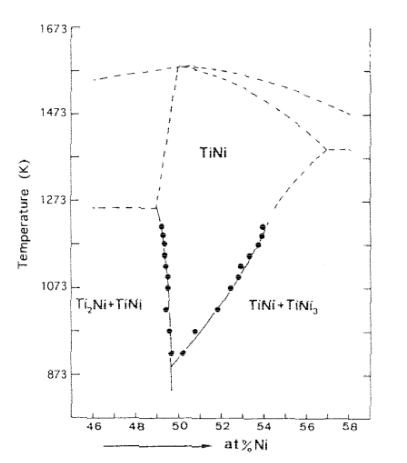
\includegraphics[scale=0.25]{img/NiTiphasediagram.png}
					\caption*{Diagrama de fases de NiTi centrado en 50\%.}
					\end{figure}
				\end{column}
				\begin{column}{.49\textwidth}
				A las propiedades ya mencionadas, la aleación $NiTi$ adicionalmente posee:
					\begin{itemize}
						\item Alta vida útil antes de sufrir fatiga
						\item Resistencia a la corrosión
						\item Biocompatible
					\end{itemize}
				\end{column}
			\end{columns}
		\end{frame}
		
	\subsection{Materiales con memoria de forma de alta temperatura}
		\begin{frame}{Materiales con memoria de forma de alta temperatura}
			Las aplicaciones actuales de los SMA están limitadas por debajo de los $100^\circ C$. Los materiales con memoria de forma de alta temperatura, abreviados como \textbf{HTSMA} (del inglés, \textbf{H}igh \textbf{T}emperature \textbf{S}hape \textbf{M}emory \textbf{A}lloys) son aquellos en los cuales la transformación martensítica sucede a $T > 100^\circ C$.
			
			Lo más común a es a $NiTi$ agregarle $Pd$ o $Pt$ en detrimento del $Ni$, pero recientemente se encontró que $Hf$ o $Zr$ en lugar del $Ti$ tienen efectos aún mayores en la temperatura a menor costo relativo.
		\end{frame}
		
	\subsection{Objetivo}
		\begin{frame}{Objetivo}
			El objetivo del presente estudio es, sabiendo que la aleación $NiTi$ presenta el efecto de memoria de forma, agregarle $Zr$ en detrimento del $Ti$ con la expectativa que las temperaturas en las cuales sucede el efecto de memoria de forma sean superiores a los 100$^\circ C$. El material se estudia en forma de láminas delgadas depositadas mediante magnetrón sputtering.
		\end{frame}
	
	\subsection{Transformación martensítica}
		\begin{frame}{Transformación martensítica}
			La causa del efecto de memoria de forma es la transformación martensítica.
			Sus propiedades son
			\begin{itemize}
				\item Transformación de estado sólido
				\item Primer orden
				\item Sin difusión atómica
				\item Desplazamiento de los átomos del orden de 1 \AA
				\item Los átomos mantienen relación con sus vecinos cercanos
			\end{itemize}
		\end{frame}
		
		\begin{frame}
			Usualmente la fase existente a mayor temperatura, llamada fase matriz o austenita, es cúbica, mientras que la fase de menor temperatura, llamada martensita debe tener menor simetría que la fase matriz, esto es, debe ser monoclínica u ortorrómbica. En el caso de $NiTi$ la austenita es la fase B2 y la martensita, la B19'.
			\begin{figure}[H]
				\subfloat[Fase B19'.]{
					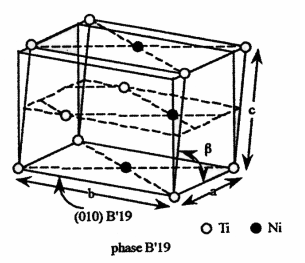
\includegraphics[scale=0.4]{img/B19pPhase.png}
				}
				\subfloat[Fase B2.]{
					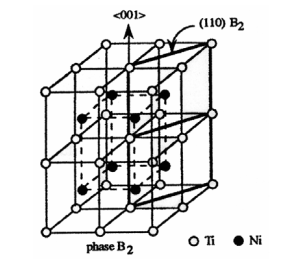
\includegraphics[scale=0.4]{img/B2Phase.png}
				}
			\end{figure}
		\end{frame}

		\begin{frame}{Temperatura de la transformación}
			\begin{columns}[T]
				\begin{column}{.49\textwidth}
					\begin{figure}
						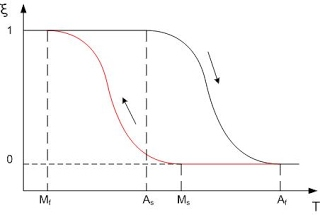
\includegraphics[scale=0.5]{img/Sma_wire.jpeg}
					\end{figure}
				\end{column}
				\begin{column}{.49\textwidth}
					\begin{figure}
						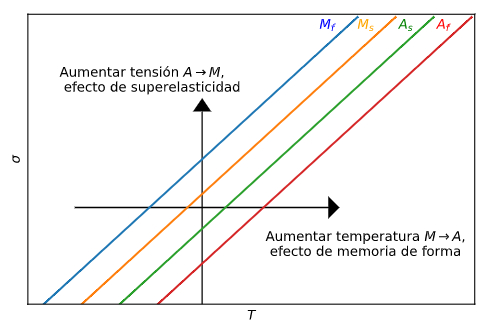
\includegraphics[scale=0.25]{img/TvsStress.png}
					\end{figure}
				\end{column}
			\end{columns}
		\end{frame}
		
		\begin{frame}{Termodinámica de la transformación}
			\begin{columns}[T] % align columns
				\begin{column}{.48\textwidth}
					\begin{figure}
						\includegraphics[scale=0.2]{img/Termo.eps}
					\end{figure}
				\end{column}
				\hfill
				\begin{column}{.48\textwidth}
				Fracción transformada ($\xi$) y energía libre de Gibbs de ambas fases como función de la temperatura en los casos: 
					\begin{itemize}
						\item si la transformación sucediera a la temperatura de equilibrio termodinámico (a) y (b)
						\item si sólo hubiera trabajo de fricción (c) y (d)
						\item si hubiera tanto trabajo de fricción como trabajo elástico (e) y (f)
					\end{itemize}
				\end{column}
			\end{columns}
		\end{frame}
		
	\subsection{Cristalización}
		\begin{frame}{Cristalización}
			\begin{figure}
				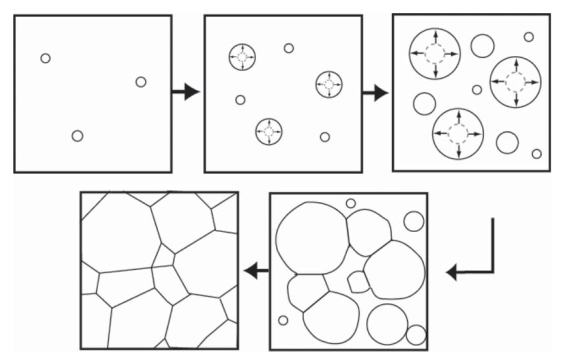
\includegraphics[scale=0.3]{img/cristalization.png}
				\caption*{Esquema de nucleación y crecimiento}
			\end{figure}
		\end{frame}

\section{Técnicas experimentales}

	\subsection{Deposición por magnetrón sputtering}
		\begin{frame}{Deposición por magnetrón sputtering}
			\begin{columns}[T]
				\begin{column}{.4\textwidth}
					\begin{figure}[H]
					\centering
					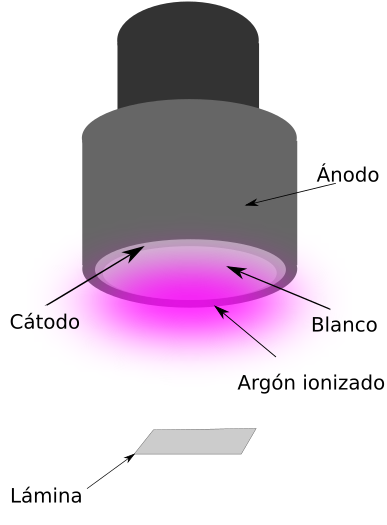
\includegraphics[scale=0.2]{img/SchemaDeposition.png}
					\caption*{Esquema magnetrón sputtering.}
					\end{figure}
				\end{column}
				\begin{column}{.58\textwidth}
					\begin{figure}[H]
					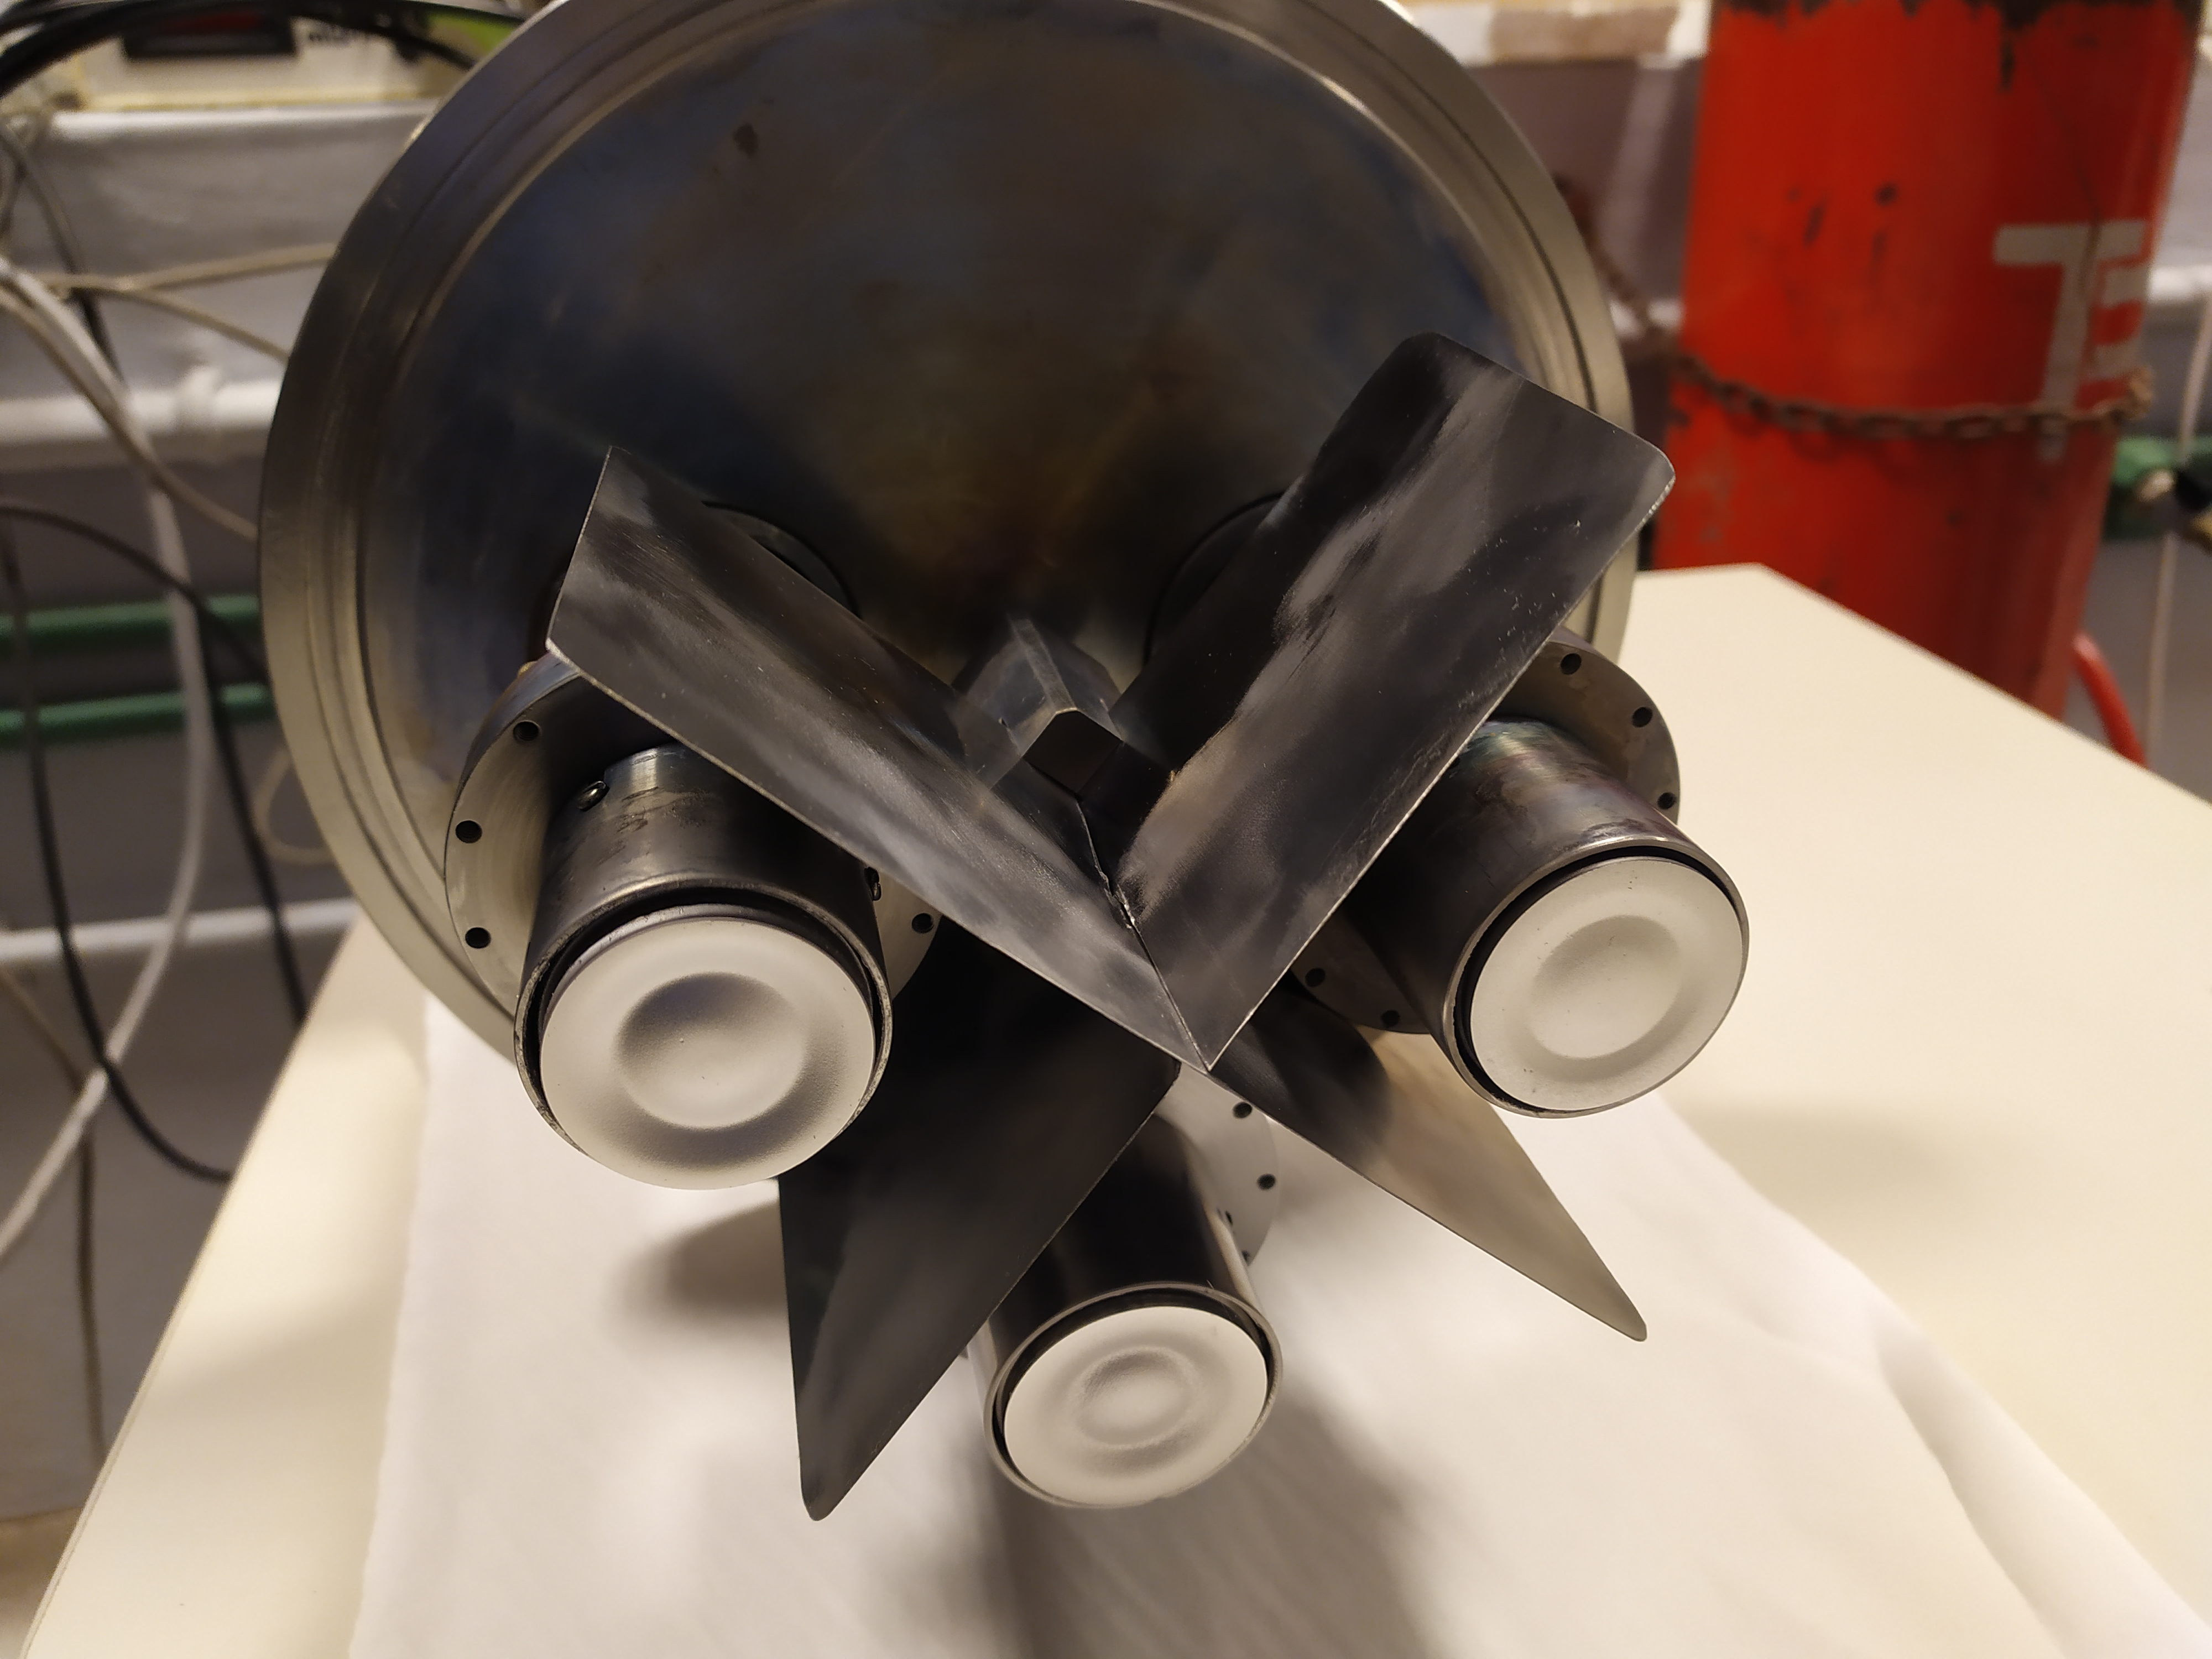
\includegraphics[scale=0.04]{img/magnetrones.jpg}
					\caption*{Magnetrones empleados.}
					\end{figure}
				\end{column}
			\end{columns}
		\end{frame}
		
		\begin{frame}{Cámara empleada}
			\begin{columns}[T]
				\begin{column}{.49\textwidth}
					\begin{figure}[H]
					\centering
					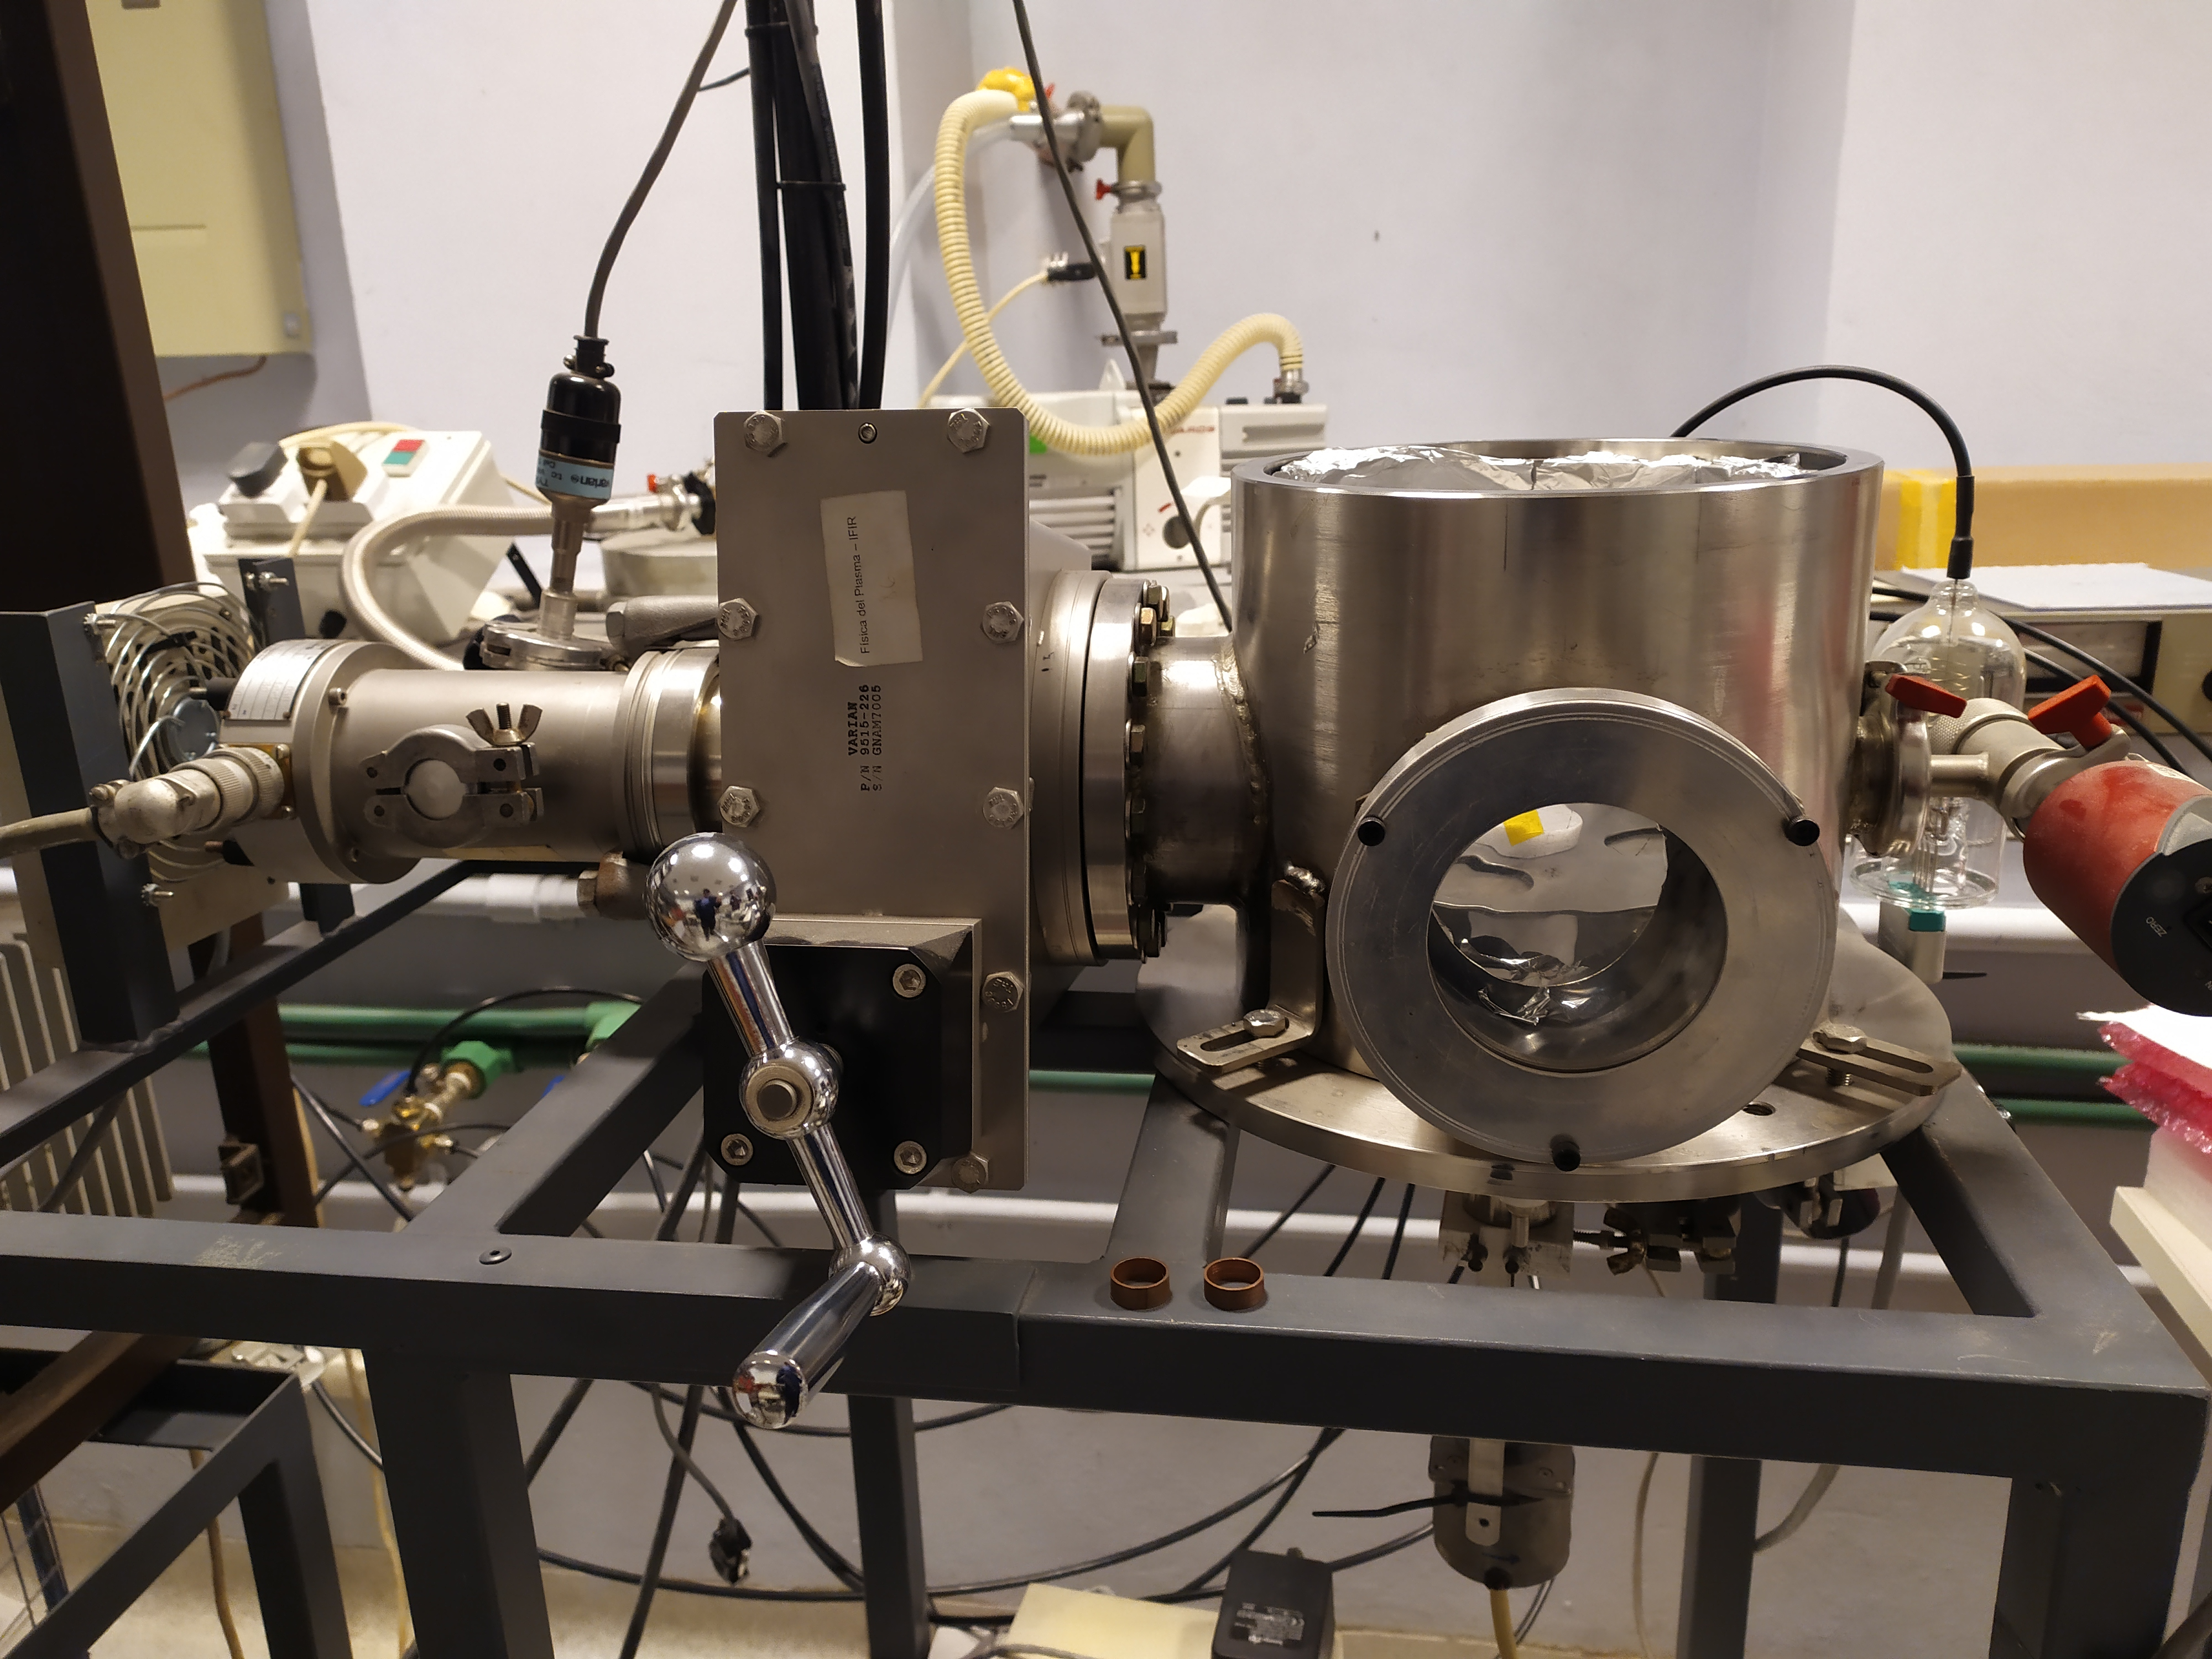
\includegraphics[scale=0.04]{img/camara.jpg}
					\caption*{Exterior de la cámara.}
					\end{figure}
				\end{column}
				\begin{column}{.49\textwidth}
					\begin{figure}[H]
					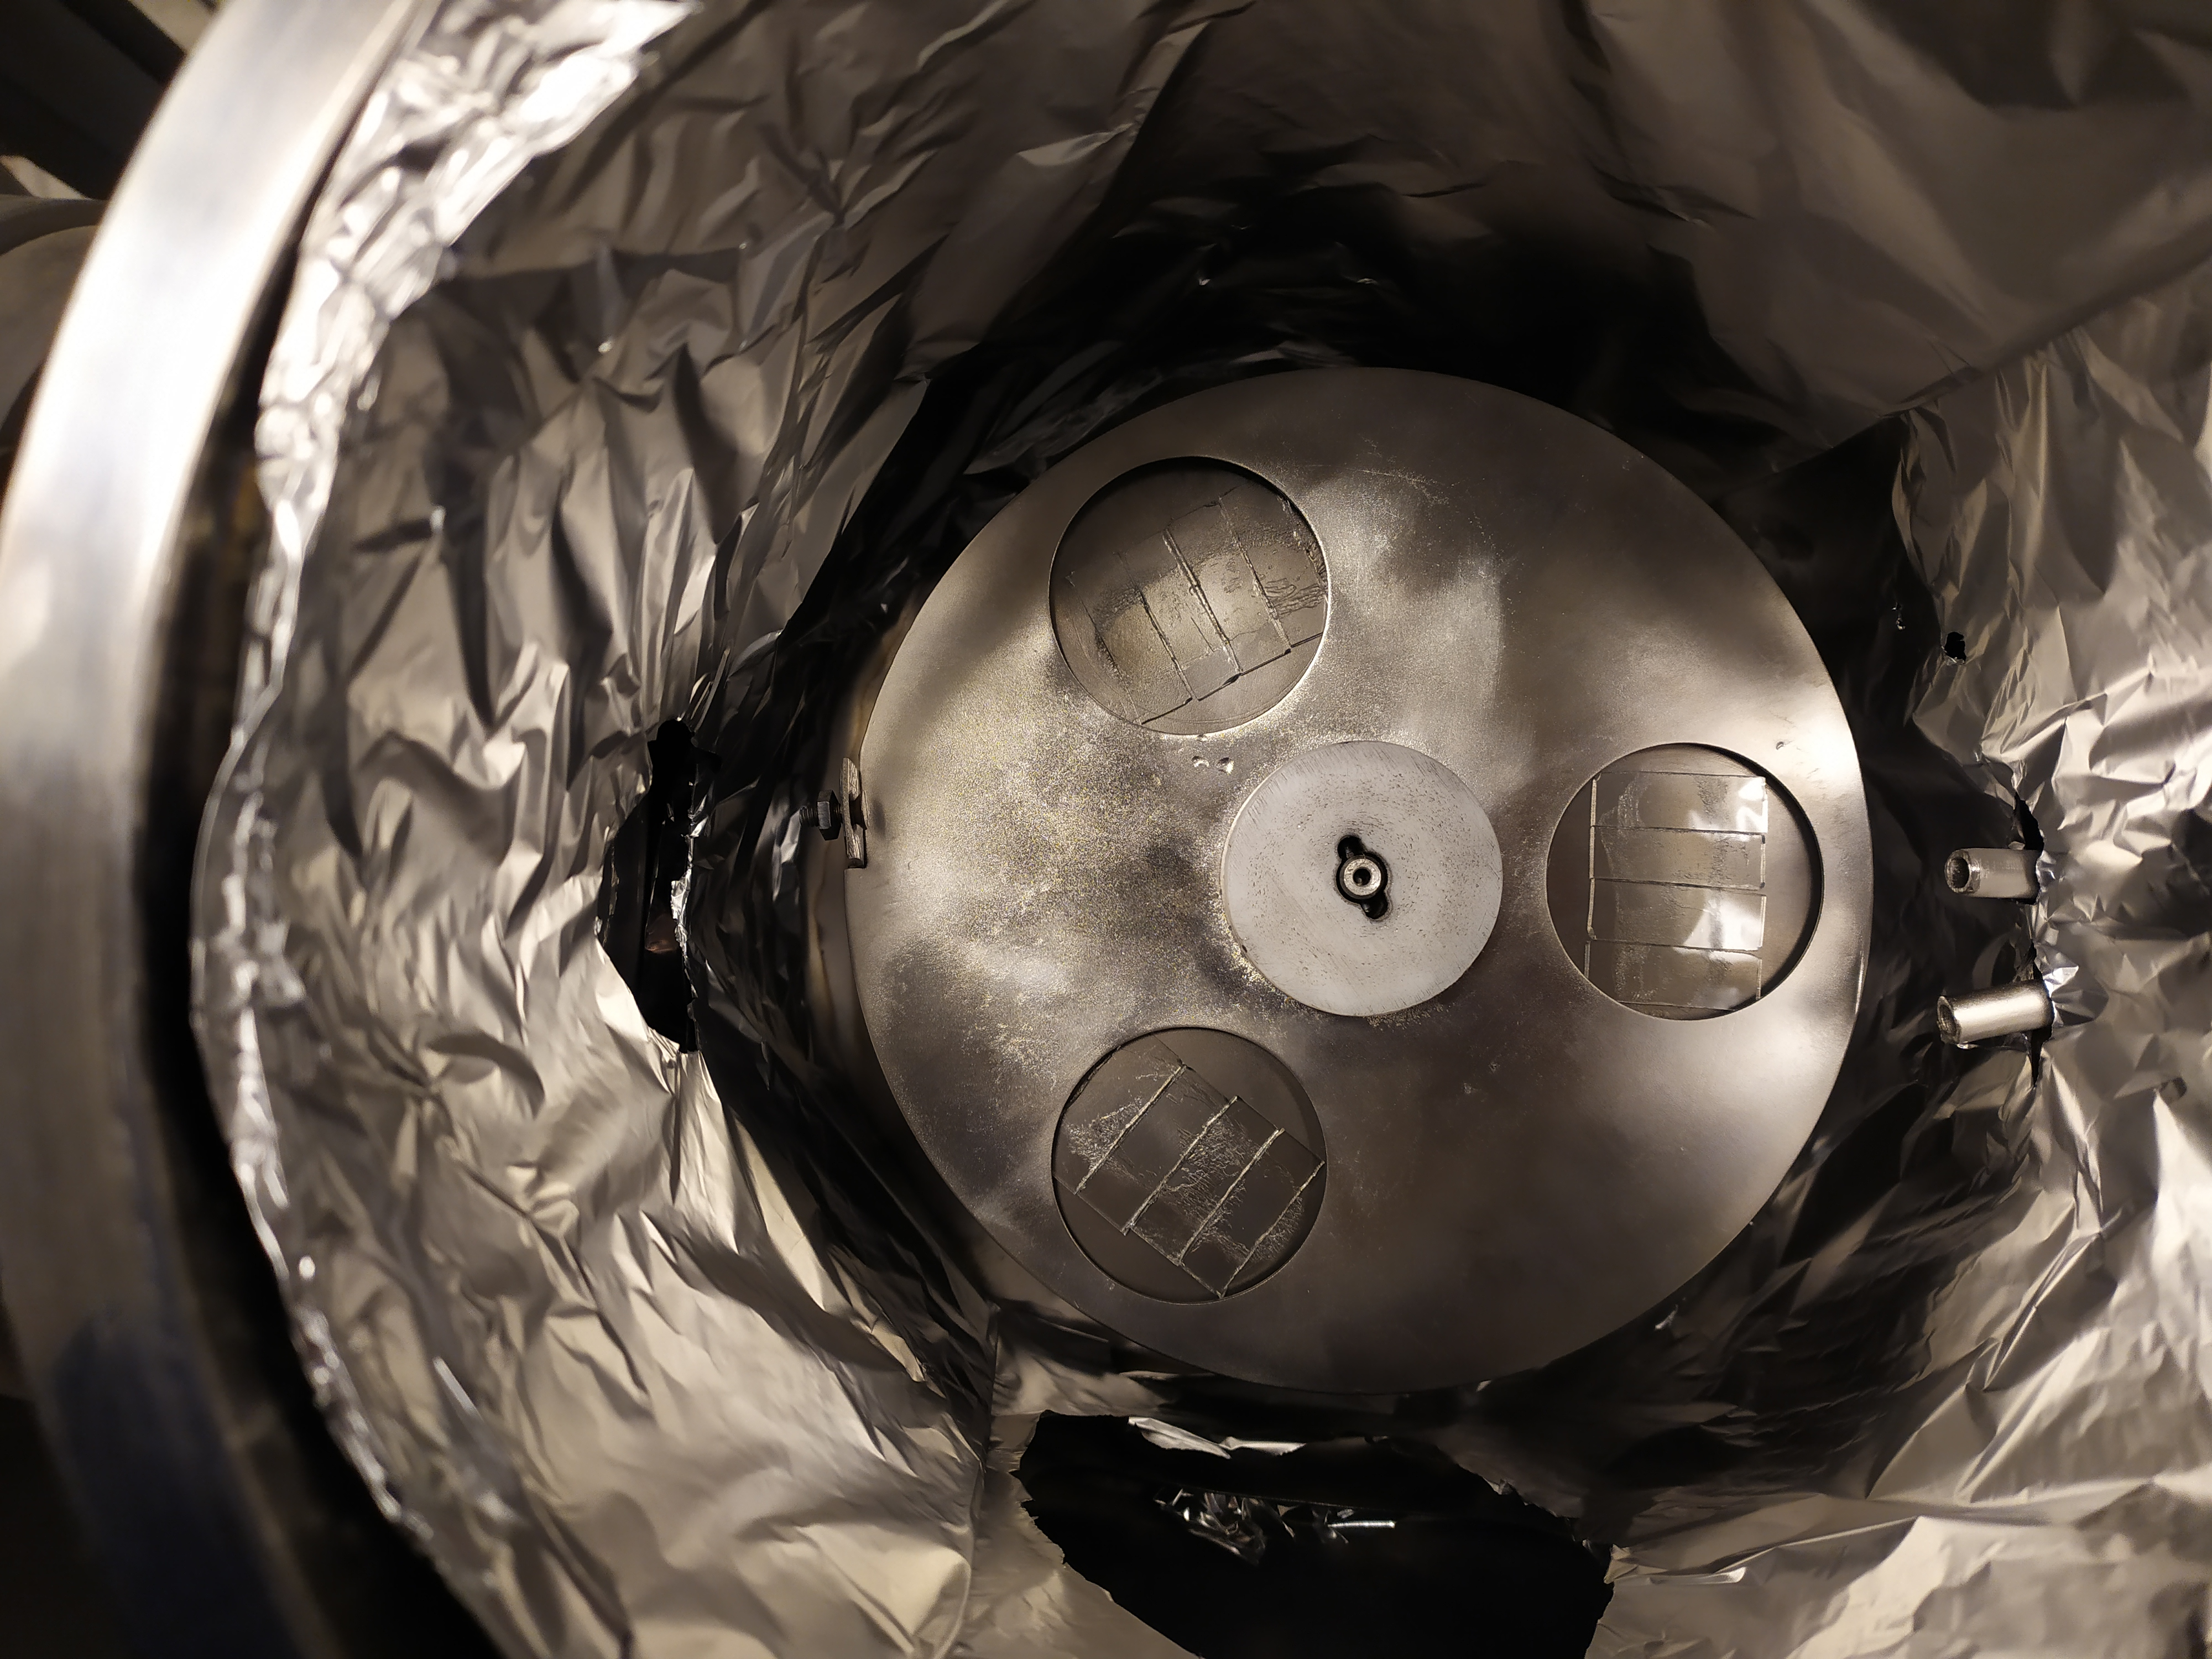
\includegraphics[scale=0.04]{img/muestras.jpg}
					\caption*{Interior de la cámara.}					
					\end{figure}
				\end{column}
			\end{columns}
		\end{frame}
	
	\subsection{Microscopía electrónica de barrido}
		\begin{frame}{Microscoṕia electrónica de barrido}
			\begin{figure}[H]
				\centering
				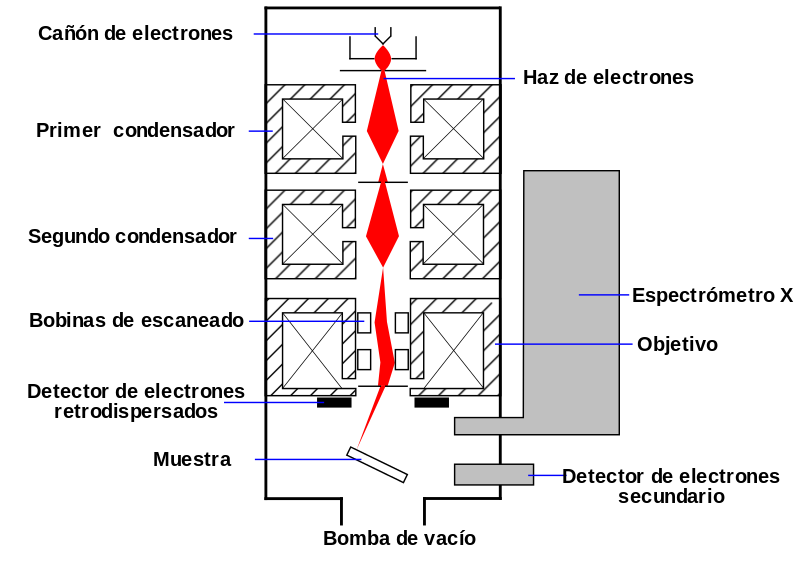
\includegraphics[scale=0.25]{img/SEM.png}
				\caption*{Esquema microscopio electrónico de barrido.}
			\end{figure}
		\end{frame}
		
	\subsection{Tratamientos térmicos}
		\begin{frame}{Tratamientos térmicos}
			\begin{figure}
				\centering
				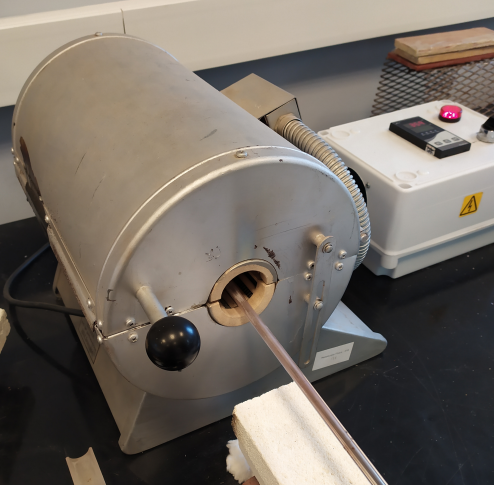
\includegraphics[scale=0.3]{img/hornito.png}
				\caption*{Horno tubular empleado para tratamientos térmicos.}				
			\end{figure}
		\end{frame}
	
	\subsection{Difracción por rayos X}
		\begin{frame}{Difracción por RX}
			\begin{columns}
				\begin{column}{.49\textwidth}
					\begin{figure}[H]
						\centering
						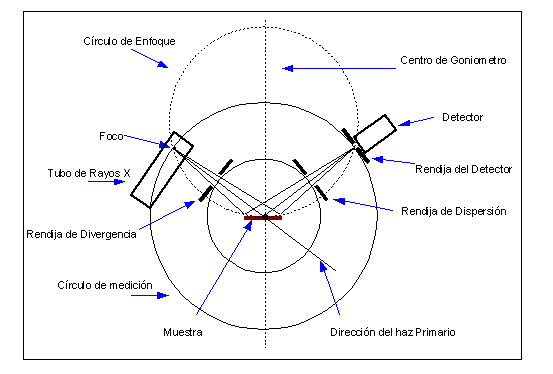
\includegraphics[scale=0.4]{img/gonio.png}
						\caption*{Esquema del dispositivo tipo Bragg-Brentano.}
					\end{figure}
				\end{column}
				\begin{column}{.49\textwidth}
					\begin{figure}[H]
						\centering
						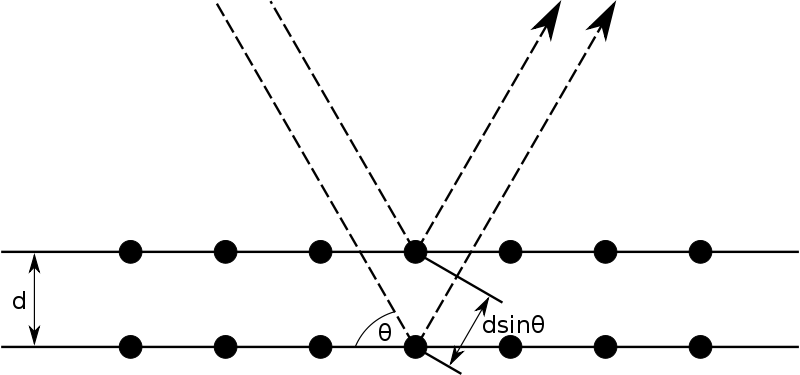
\includegraphics[scale=0.1]{img/Bragg.png}
						\caption*{Esquema del dispositivo tipo Bragg-Brentano.}
					\end{figure}
				\end{column}
			\end{columns}
		\end{frame}
	
	\subsection{Microscopía electrónica de transmisión}
		\begin{frame}{Microscopía electrónica de transmisión}
			\begin{figure}[H]
				\centering
				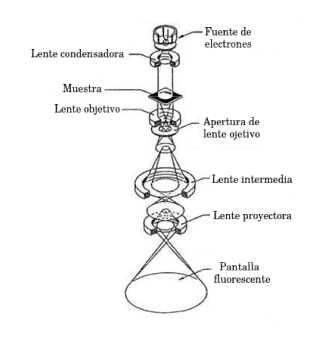
\includegraphics[scale=0.4]{img/TEM.png}
				\caption*{Esquema del tubo de un microscopio electrónico de 							  transmisión.}
			\end{figure}
		\end{frame}

	\subsection{Calorimetría diferencial de barrido}
		\begin{frame}
			\begin{figure}[H]
				\centering
				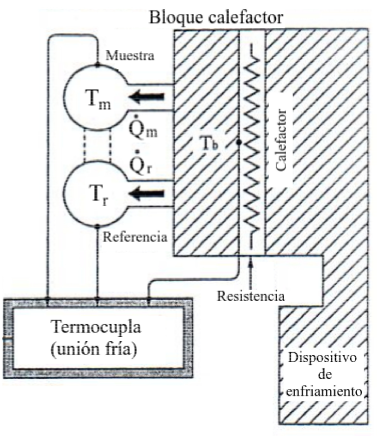
\includegraphics[scale=0.3]{img/DSCscheme.png}
				\caption*{Esquema del DSC empleado.}
			\end{figure}
		\end{frame}

	\subsection{Resistividad por el método de cuatro puntas}
		\begin{frame}
			\begin{columns}
				\begin{column}{.49\textwidth}
					\begin{figure}[H]
						\centering
						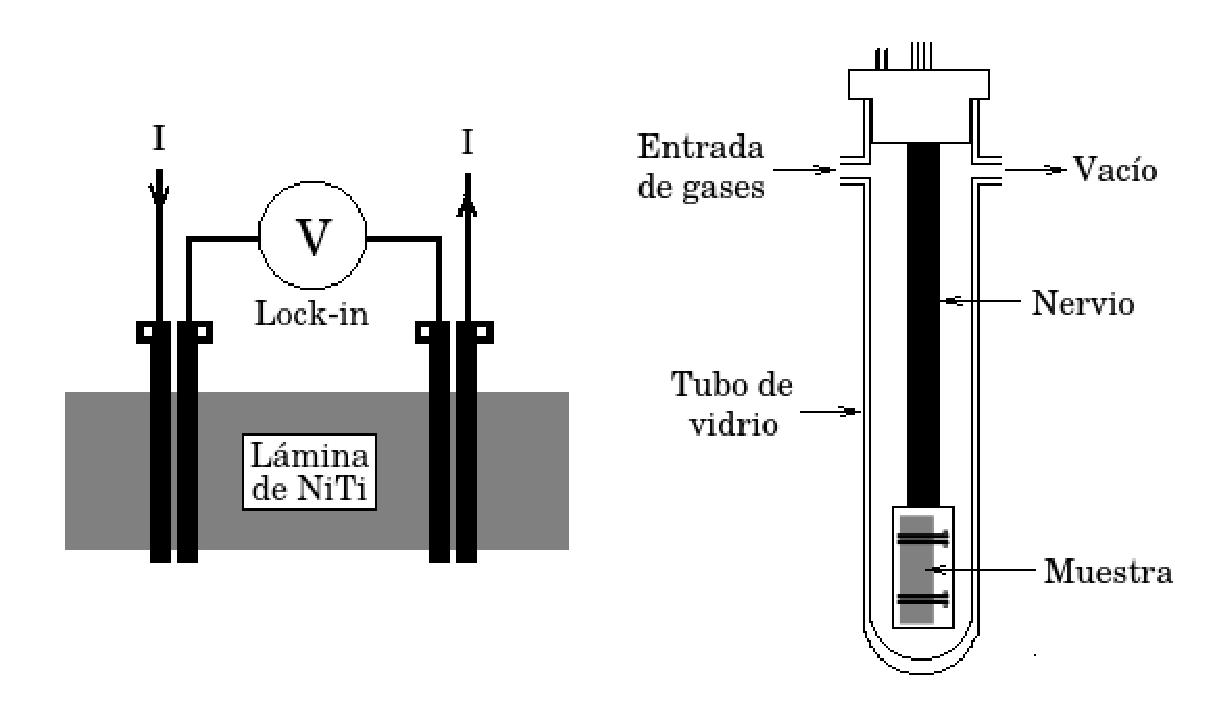
\includegraphics[scale=0.3]{img/resistividad.eps}
						\caption*{Esquema del sistema empleado para el método de 								 resistividad por cuatro puntas.}
					\end{figure}
				\end{column}
				\begin{column}{.49\textwidth}
					\begin{figure}[H]
						\centering
						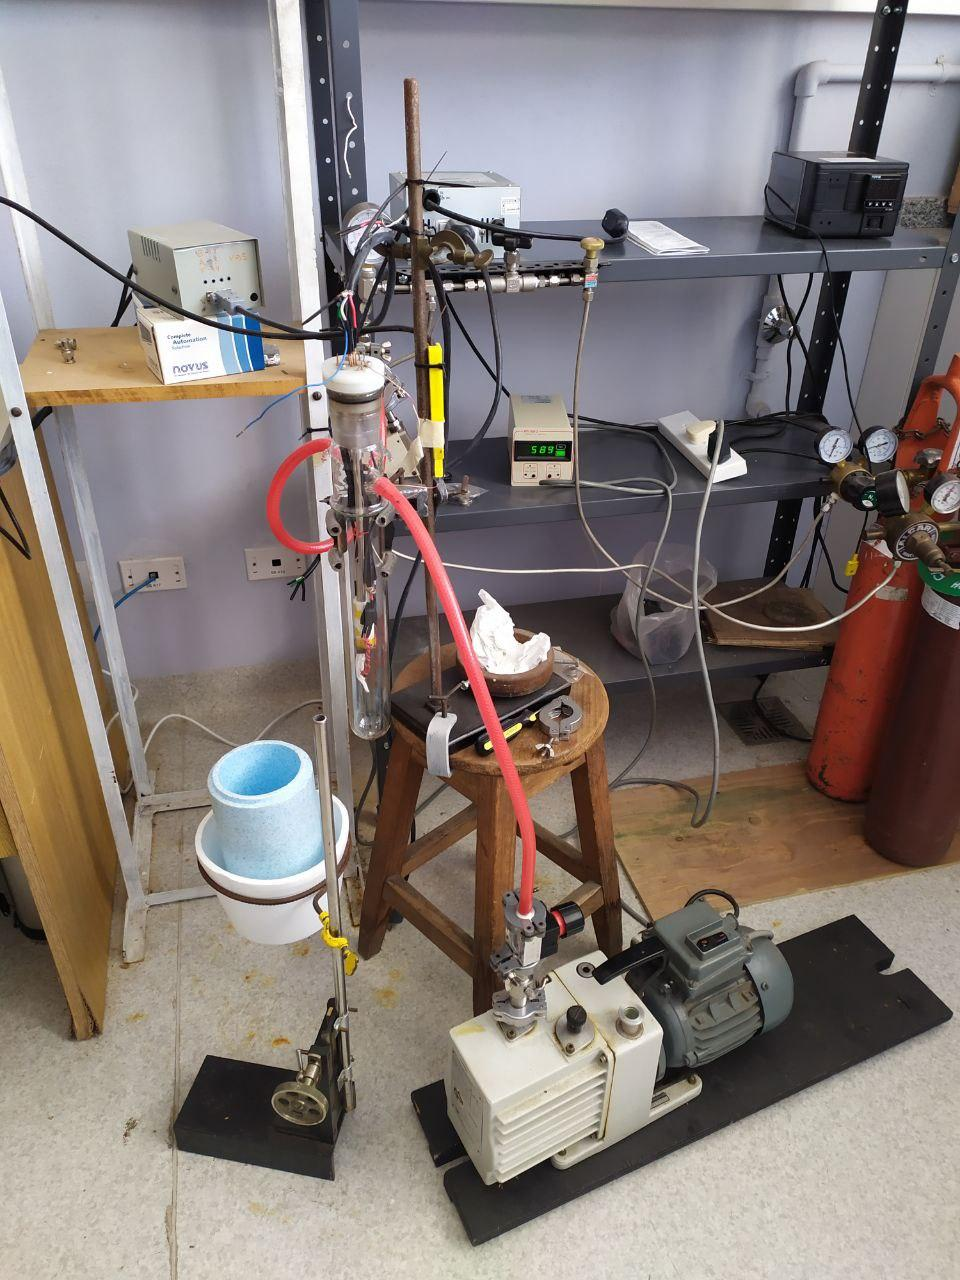
\includegraphics[scale=0.1]{img/resistividad.jpg}
						\caption*{Resistividad por cuatro puntas.}
					\end{figure}
				\end{column}
			\end{columns}
		\end{frame}
	
\section{Resultados obtenidos}
	\subsection{Deposición de las láminas}
		\begin{frame}
			\begin{figure}
				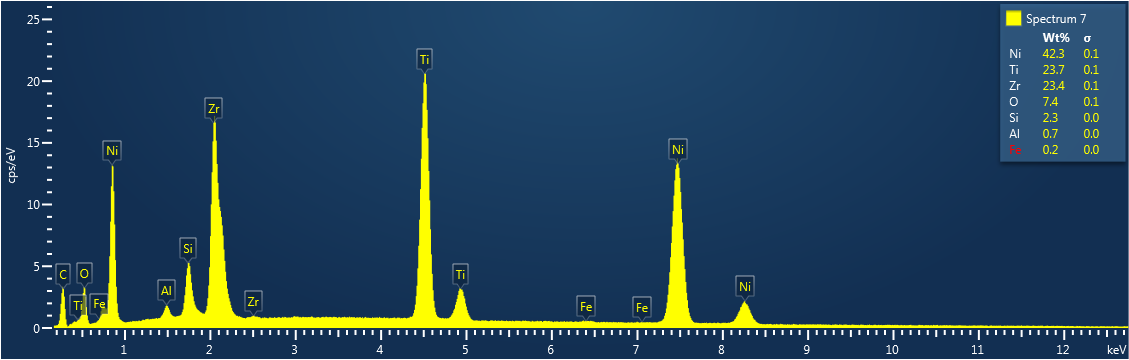
\includegraphics[scale=0.25]{img/SEMAllElements.png}
				\caption*{Resultados de una medición con SEM sin filtrar elementos.}
			\end{figure}
			\begin{table}[H]
				\centering
				\begin{tabular}{c|c|c|}
				\cline{2-3}
				\multicolumn{1}{l|}{} & Primera Deposición & Segunda Deposición \\ \hline
				\multicolumn{1}{|c|}{Ti{[}\%at{]}} & 30,8 $\pm$ 0,6 & 33,2 $\pm$ 0,5 \\ \hline
				\multicolumn{1}{|c|}{Ni{[}\%at{]}} & 50,4 $\pm$ 0,2 & 46 $\pm$ 1 \\ \hline
				\multicolumn{1}{|c|}{Zr{[}\%at{]}} & 18,9 $\pm$ 0,5 & 20,8 $\pm$ 0,4 \\ \hline
				\end{tabular}
				\caption*{Composición determinada para ambas deposiciones.}
				\label{compositionAvg}
			\end{table}
		\end{frame}

	\subsection{Energía de activación}
	\begin{frame}{Energía de activación}
		\begin{figure}
			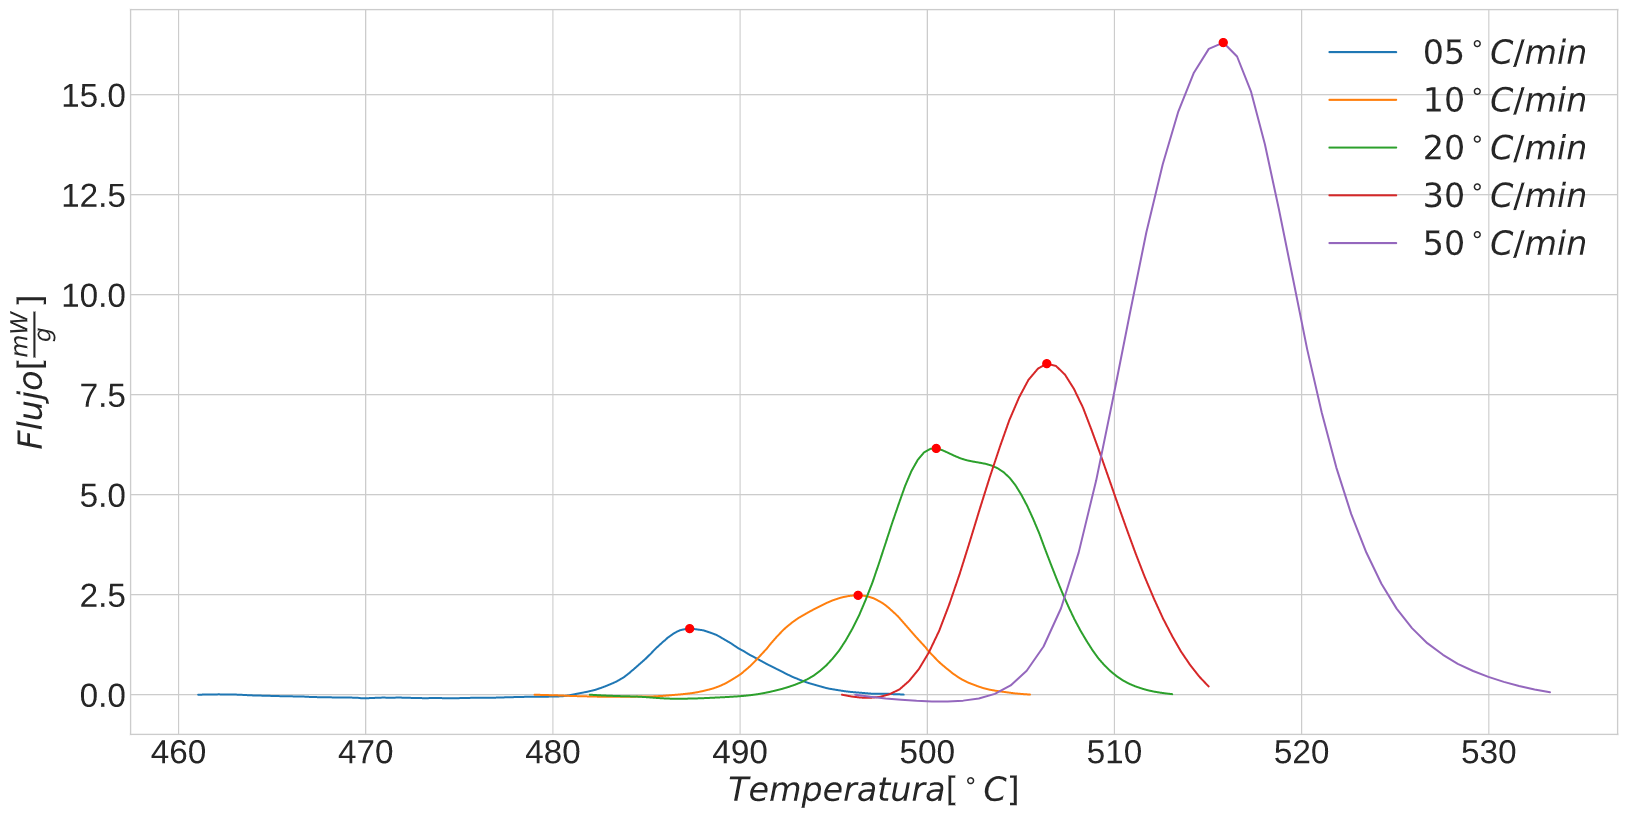
\includegraphics[scale=0.1]{img/DSCPeaks.png}
			\caption*{Flujo de calores a distintas velocidades de calentamiento.}
		\end{figure}
	\end{frame}
	
	\begin{frame}
		\begin{columns}
			\begin{column}{.49\textwidth}
				\begin{figure}
					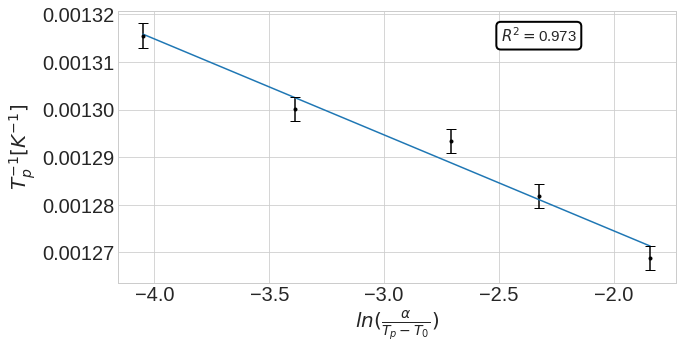
\includegraphics[scale=0.2]{img/Augis_bennet.png}
					\caption*{Regresión por el método de Augis-Bennet. $E_c = 410 \pm 30$ kJ}
				\end{figure}
			\end{column}
			\begin{column}{.49\textwidth}
				\begin{figure}
					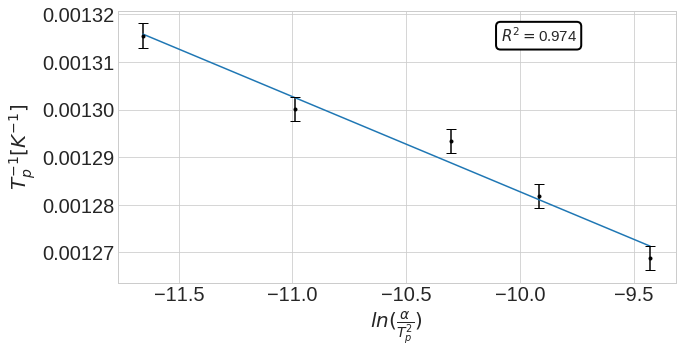
\includegraphics[scale=0.2]{img/Kissinger.png}
					\caption*{Regresión por el método de Kissinger. $E_c = 420 \pm 30$ kJ}				
				\end{figure}
			\end{column}
		\end{columns}
	\end{frame}
	
	\begin{frame}
		\begin{table}[H]
			\centering
			\begin{tabular}{|c|c|c|}
				\hline
				Composición & \begin{tabular}[c]{@{}c@{}}Energía de \\ activacion {[}kJ/mol{]}\end{tabular} & Método \\ \hline
				$Ni_{48,89}Ti_{40,50}Zr_{10,61}$ & 417,2  & composición en cinta\\ \hline
				$Ni_{48,71}Ti_{35,59}Zr_{15,70}$ & 432,9 & composición en cinta\\ \hline
				$Ni_{48,25}Ti_{31,26}Zr_{20,49}$ & 482,4 & composición en cinta\\ \hline
				$Ni_{47,95}Ti_{26,72}Zr_{25,33}$ & 465,8 & composición en cinta\\ \hline
				$Ni_{49,40}Ti_{19,96}Zr_{30,64}$ & 445,7 & composición en cinta\\ \hline
				$Ni_{49,6}Ti_{30,9}Zr_{19,5}$ & 449 $\pm$ 5 & melt spinning\\ \hline
			\end{tabular}
			\caption*{Valores reportados por Xiaoyang Yi et al para la energía de activación para distintas composiciones en cinta.}
			\label{XiaoyangYiValues}
		\end{table}

%Por otra parte, Malvasio en 2017 \citep{Malvasio}, en láminas delgadas obtenidas por deposición mediante magnetrón sputtering en la aleación binaria ($Ni_{54,2}Ti_{45,8}$), obtuvo una energía de activación de $E_c = 300 \pm 30 kJ/mol$ tanto por el método de Kissinger como por el método de Augis-Bennet.
%
%En el presente trabajo se determinó la energía de activación de láminas delgadas de $NiTiZr$ producidas por magnetrón sputtering para la composición rica en $Ni$ ($Ni_{50,4}Ti_{30,8}Zr_{18,9}$) y se obtuvieron valores de $E_c = 420 \pm 30$ kJ por el método de Kissinger y de $E_c = 410 \pm 30$ kJ por el método de Augis-Bennet. Si bien estos valores son levemente inferiores a los determinados por Xiaoyang Yi et al., son notoriamente mayores que los obtenidos en la aleación binaria. La leve diferencia entre los valores determinados en este trabajo con los valores obtenidos por Xiaoyang Yi et al. puede ser entendida teniendo en cuenta las diferentes técnicas de producción. Estas diferencias en los valores de la energía de activación causado por los procesos de producción, ya fueron mostrados en la aleación binaria.
	\end{frame}

	\subsection{Pobres en $Ni$}
		\begin{frame}{Fases obtenidas}
			\begin{figure}[H]
				\captionsetup[subfloat]{labelformat=empty}
				\subfloat[Muestra a $500 ^\circ C$]{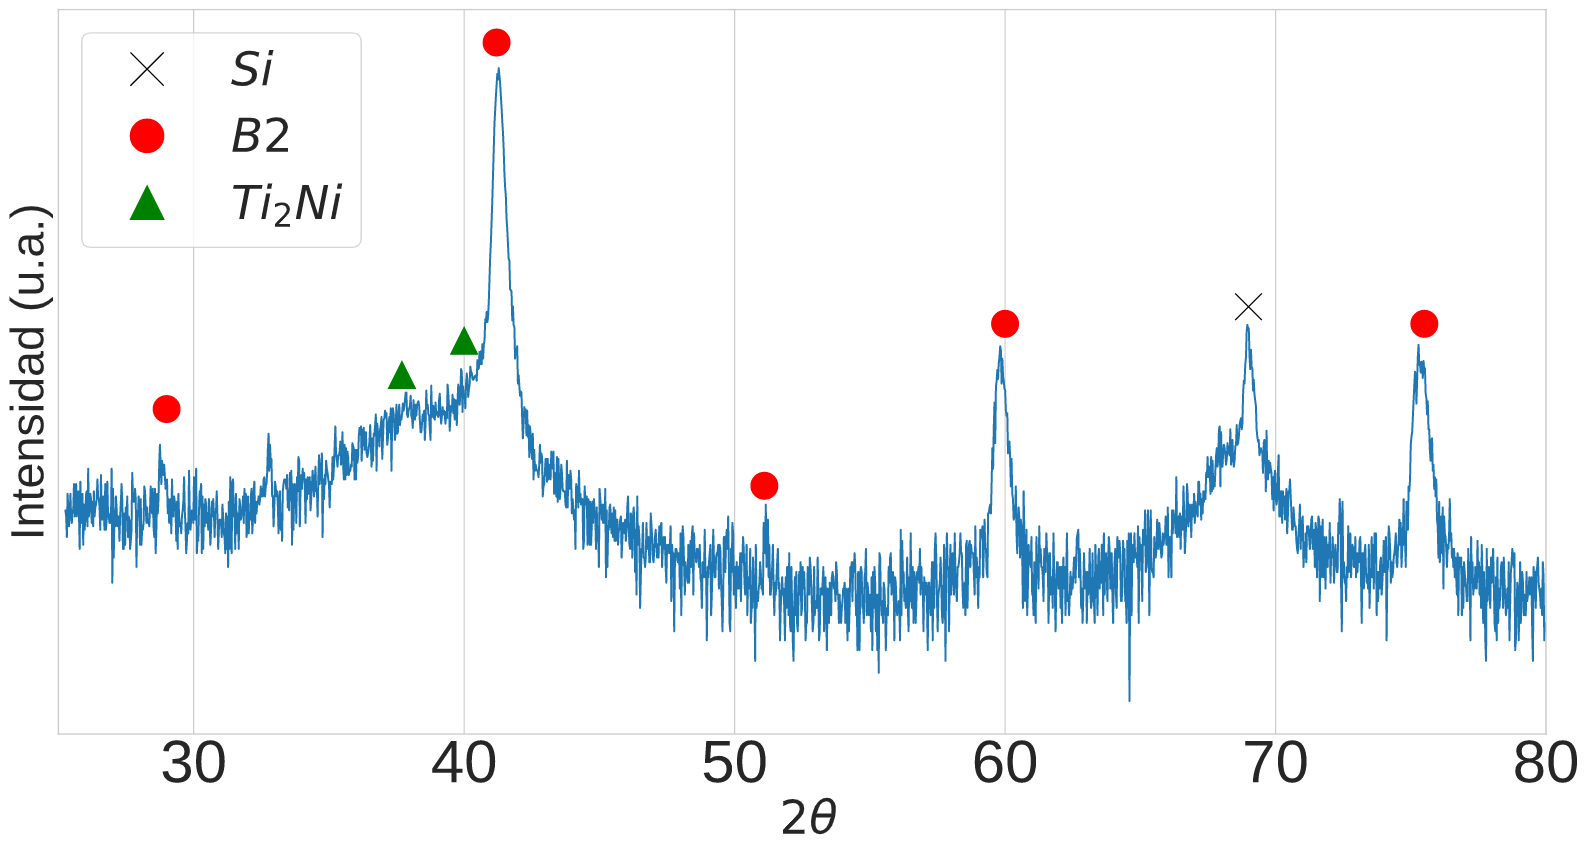
\includegraphics[scale=0.09]{img/RX/NiPoor_500.png}} \qquad
				\subfloat[Muestra a $600 ^\circ C$]{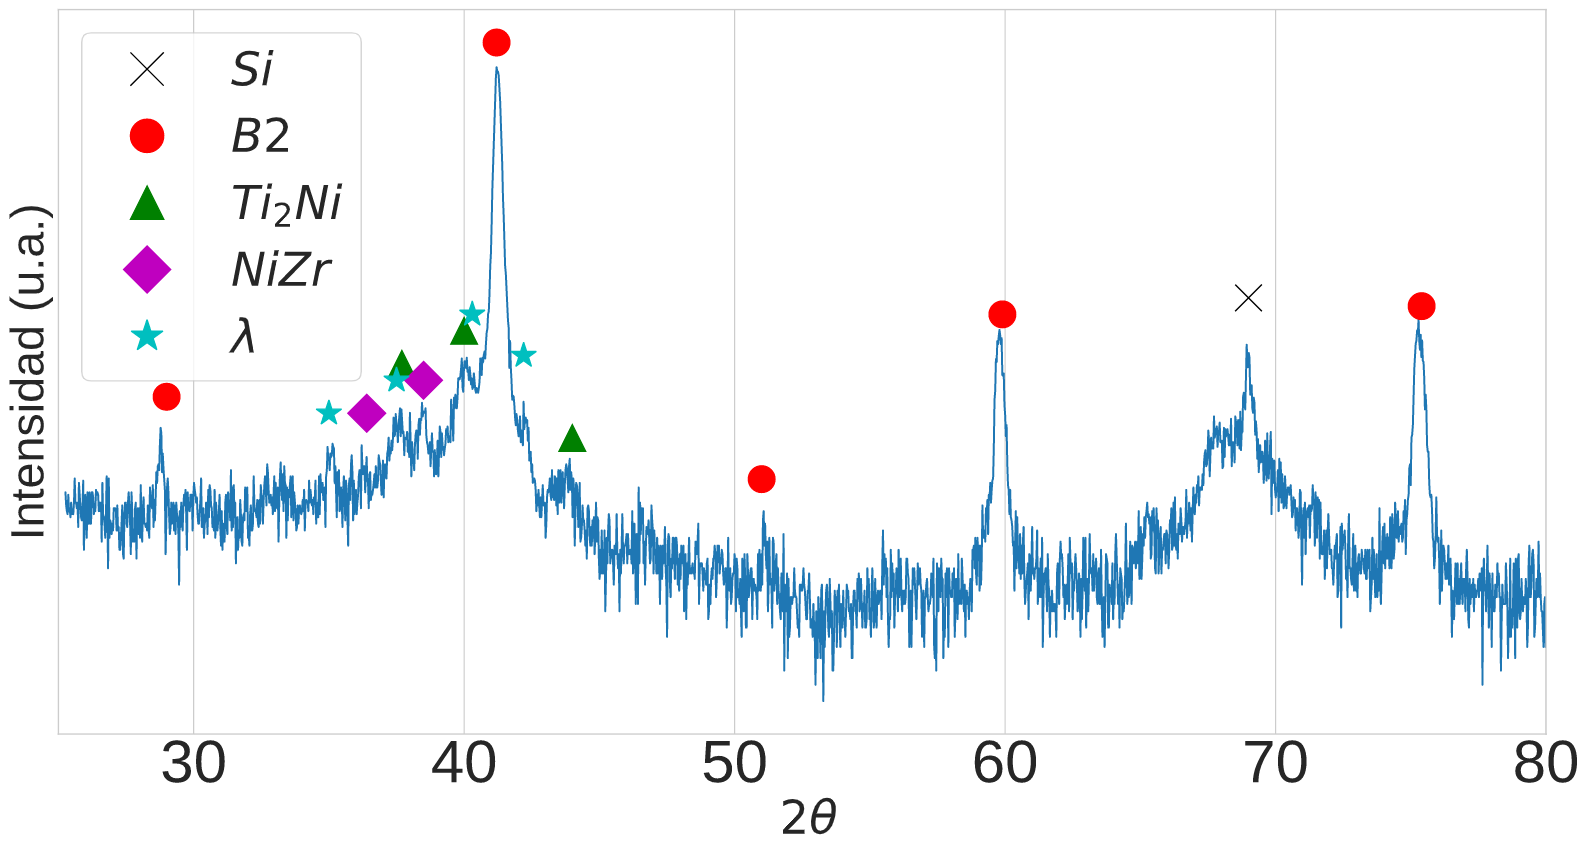
\includegraphics[scale=0.09]{img/RX/NiPoor_600.png}} \\
				\subfloat[Muestra a $700 ^\circ C$]{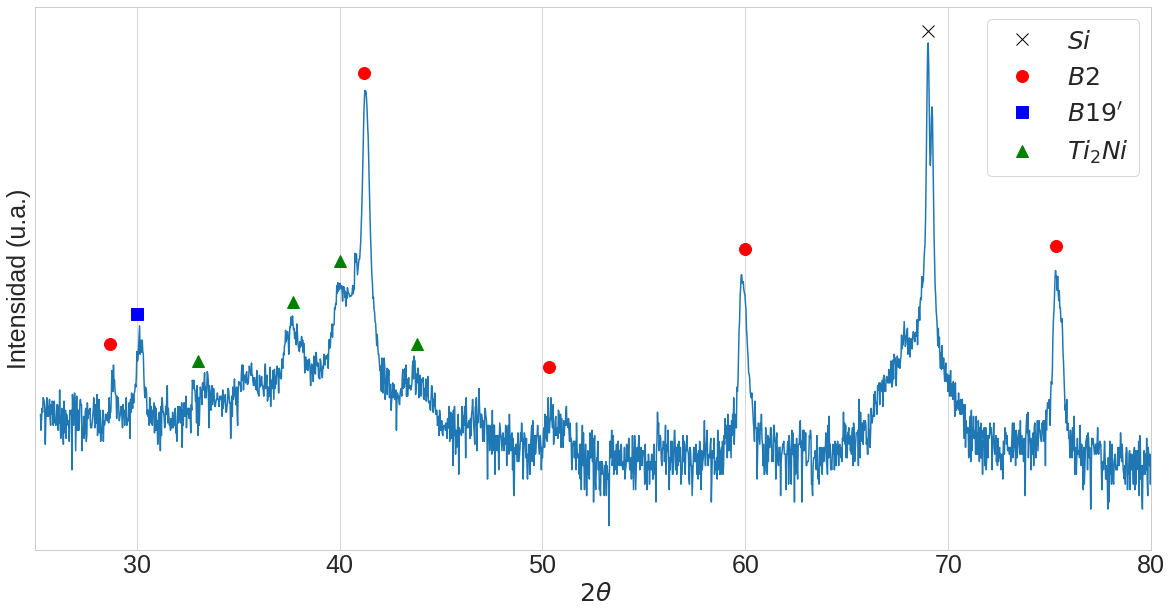
\includegraphics[scale=0.09]{img/RX/NiPoor_700.png}} \qquad
				\subfloat[Muestra a $800 ^\circ C$]{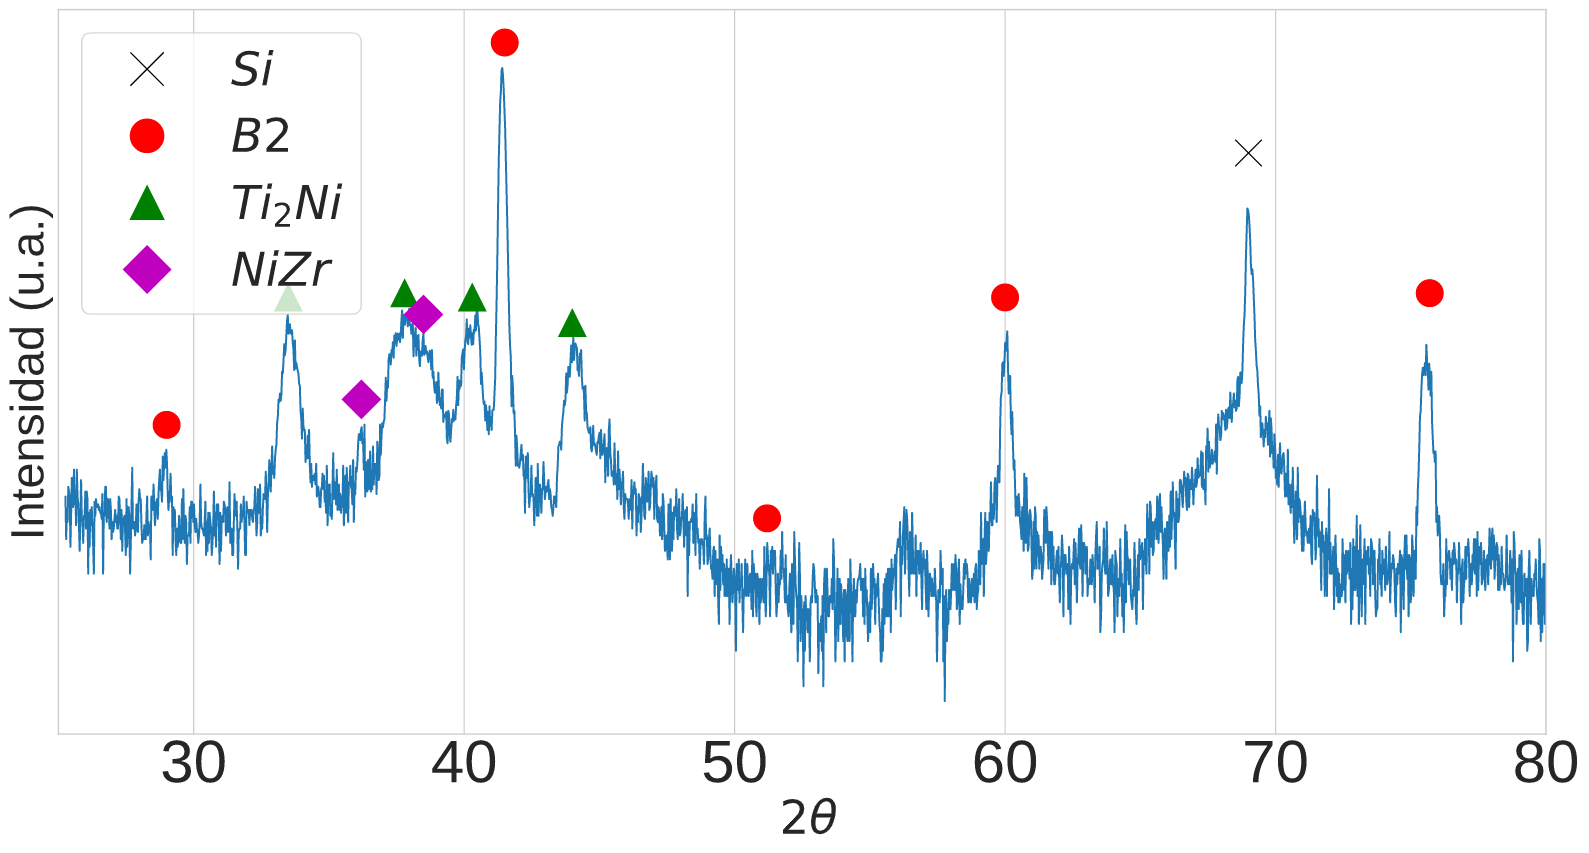
\includegraphics[scale=0.09]{img/RX/NiPoor_800.png}} \\
				\caption*{Patrones de difracción para las muestras pobres en $Ni$.}
				\label{RXNiPoor}
			\end{figure}		
		\end{frame}
		
		\begin{frame}{Imágenes obtenidas por TEM}
			\begin{figure}[H]
			\captionsetup[subfloat]{labelformat=empty}
				\centering
				\subfloat[Muestra a $500 ^\circ C$]{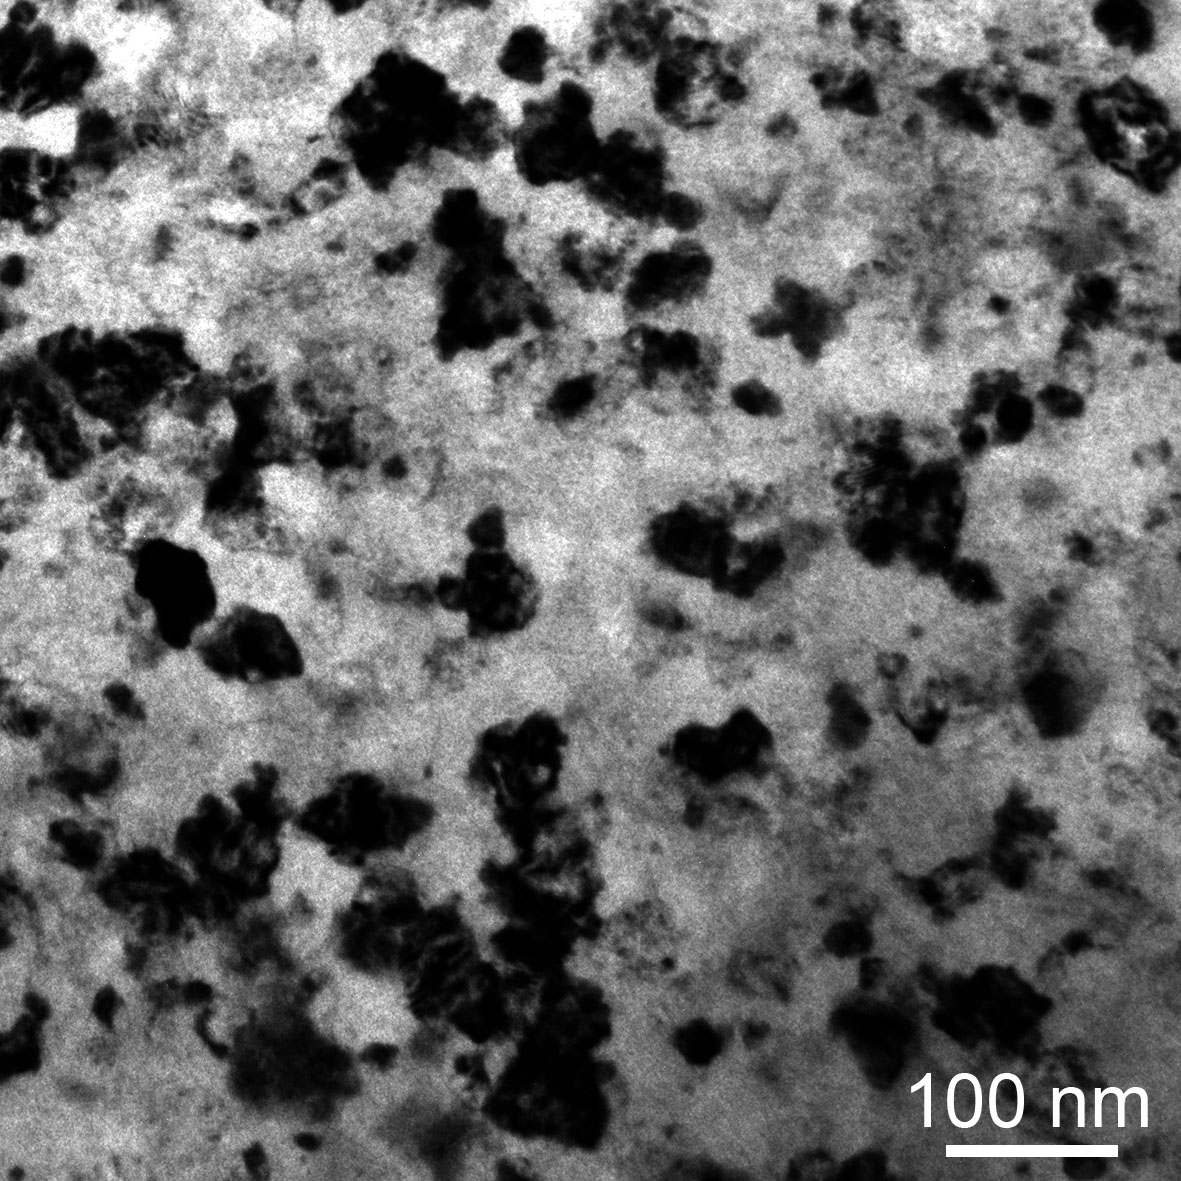
\includegraphics[scale=0.2]{img/TEM/Fig24a.jpg}} \qquad
				\subfloat[Muestra a $600 ^\circ C$]{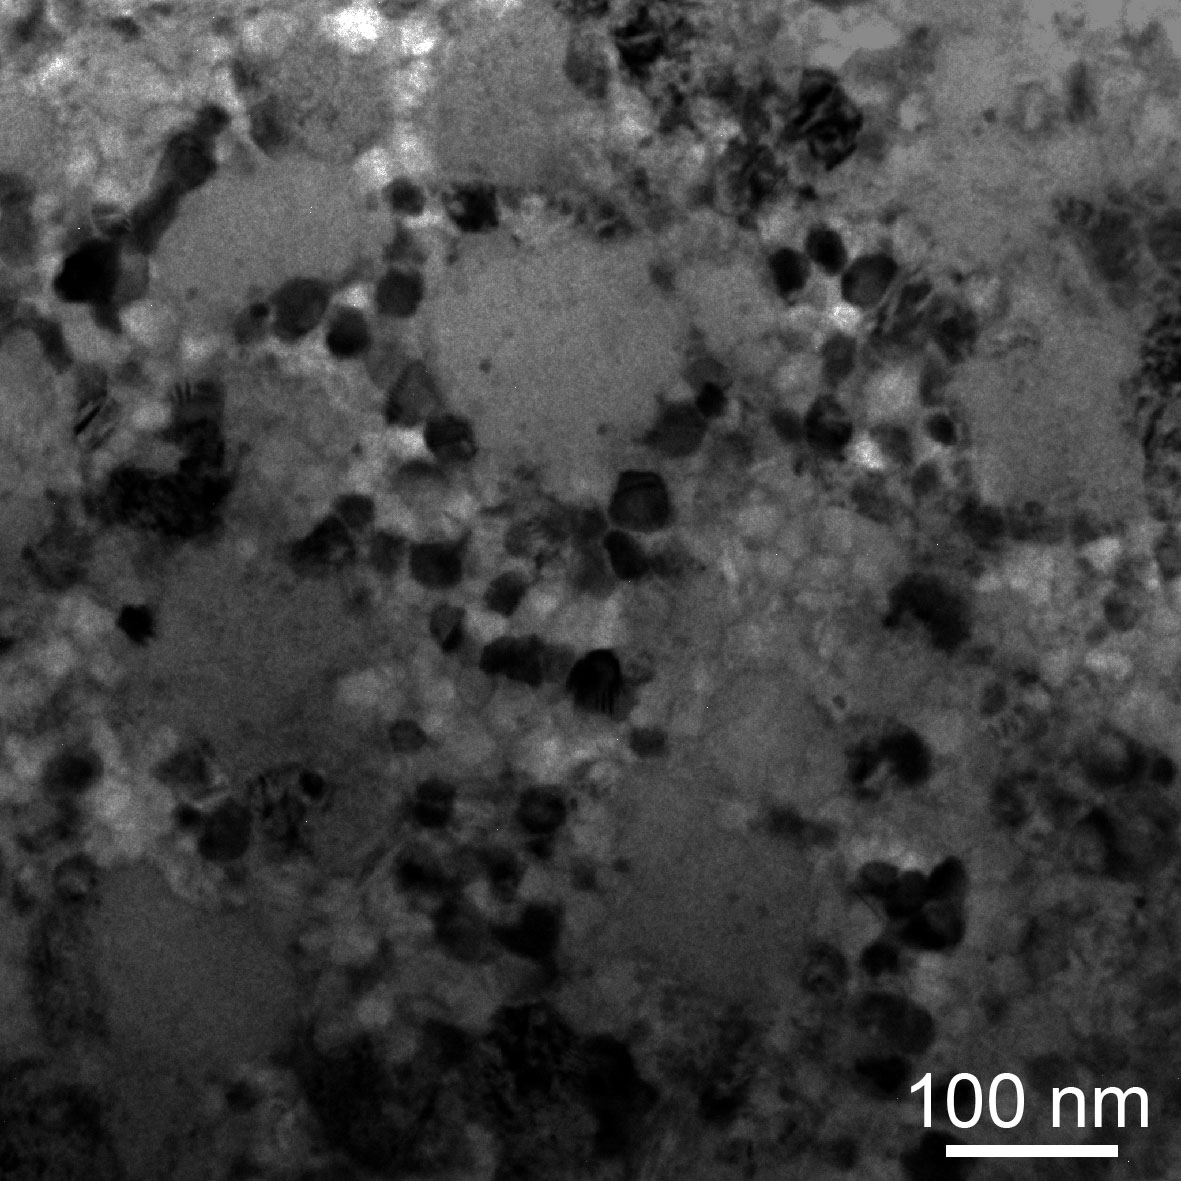
\includegraphics[scale=0.2]{img/TEM/Fig24b.jpg}} \\
				\subfloat[Muestra a $700 ^\circ C$]{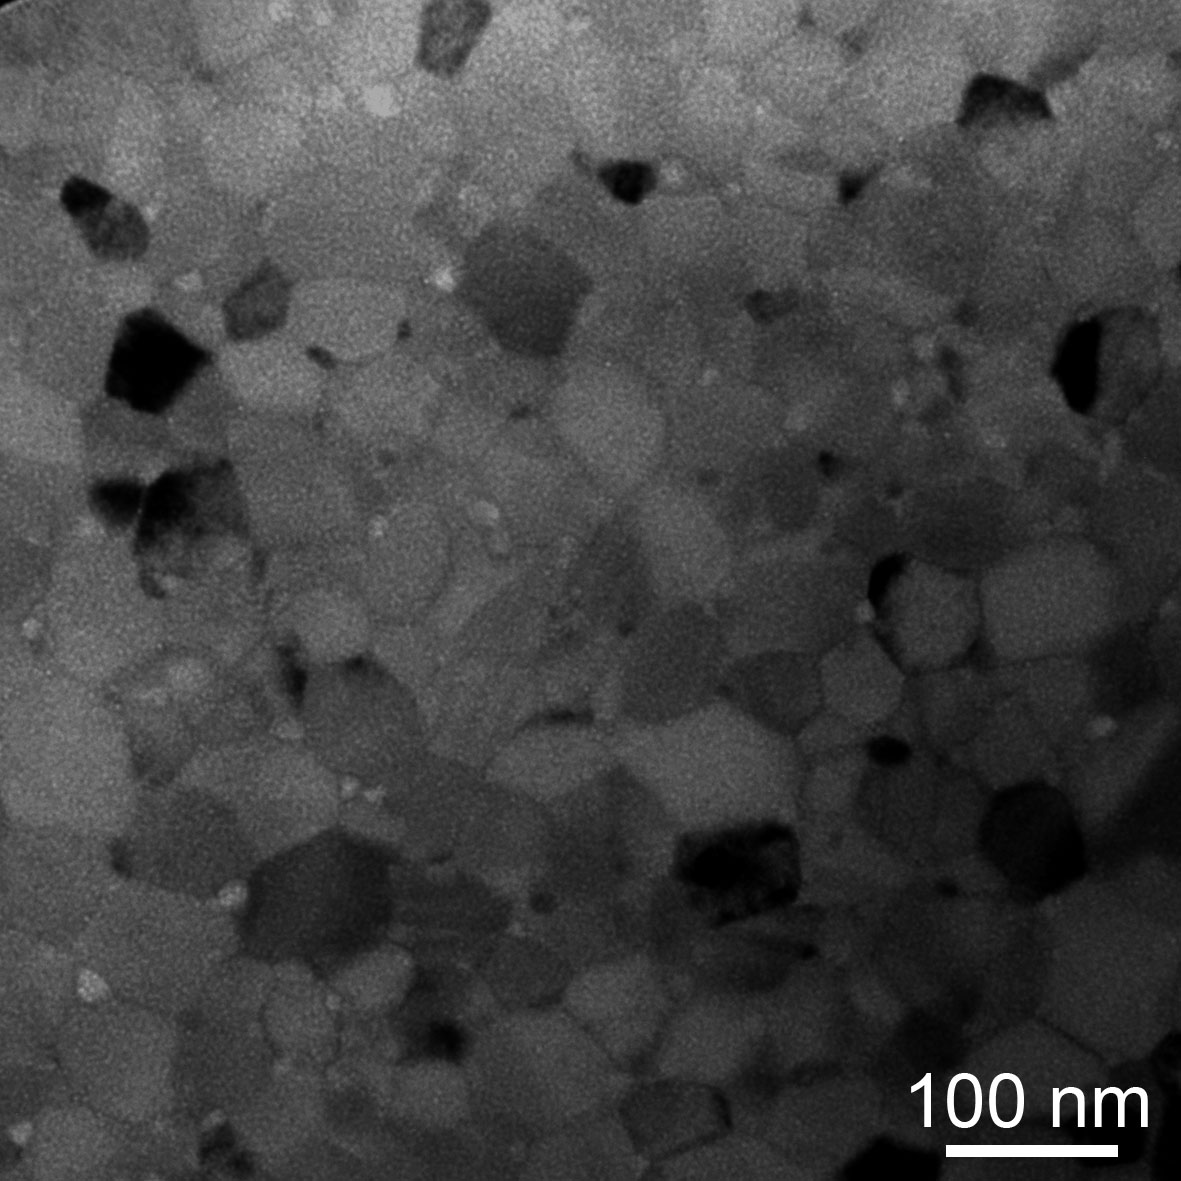
\includegraphics[scale=0.2]{img/TEM/Fig24c.jpg}} \qquad
				\subfloat[Muestra a $800 ^\circ C$]{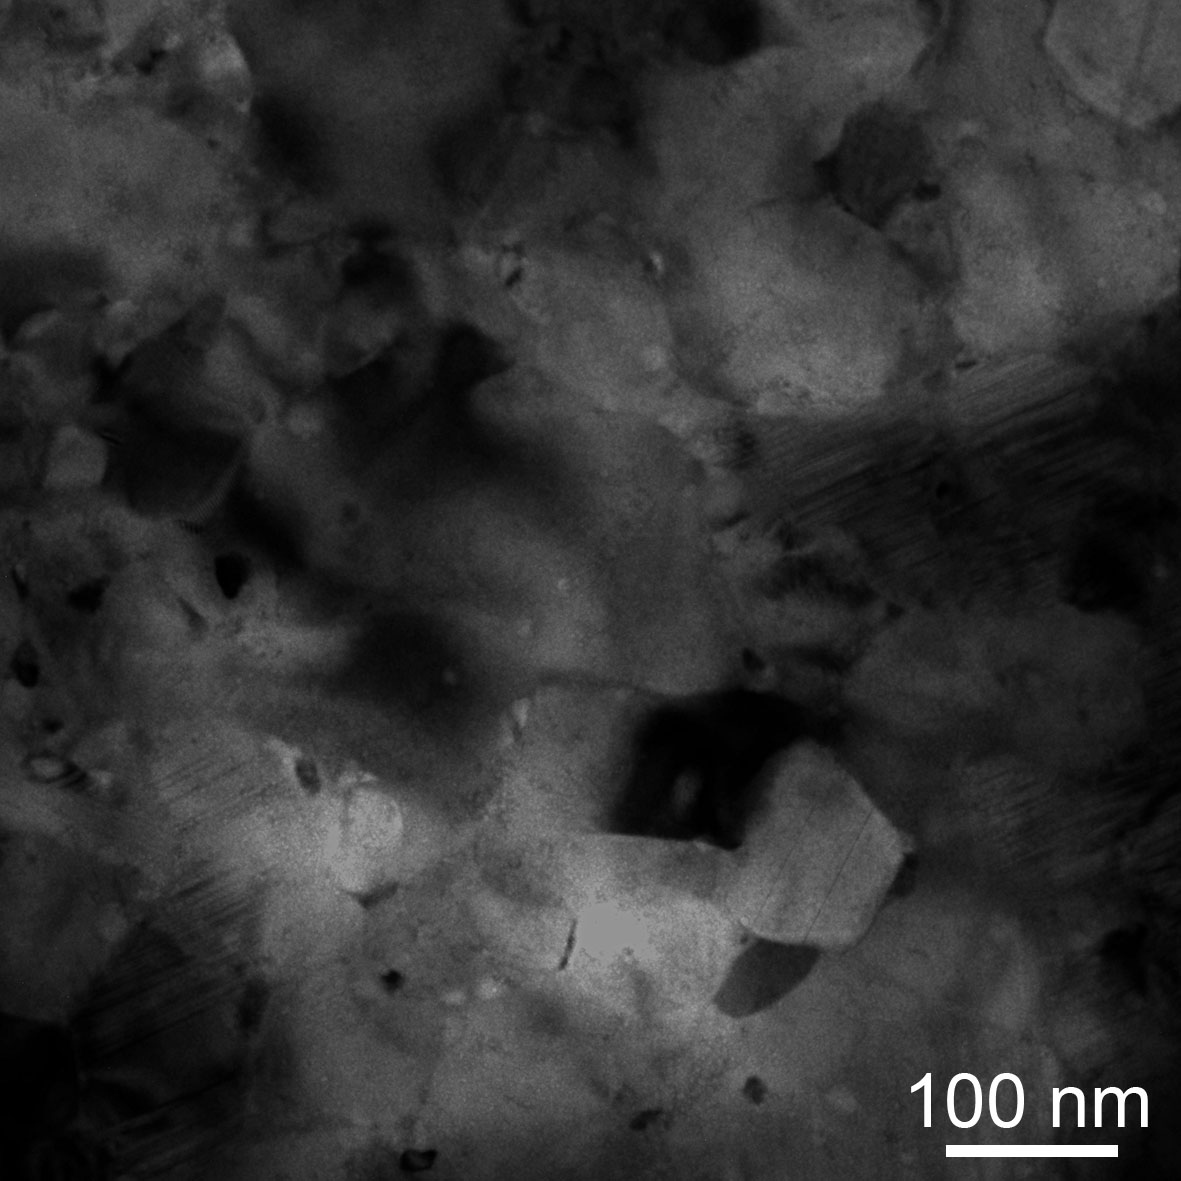
\includegraphics[scale=0.2]{img/TEM/Fig24d.jpg}}
				\caption*{Imágenes de TEM para las muestras pobres en $Ni$.}
			\end{figure}
		\end{frame}
		
		\begin{frame}{Curvas de DSC}
			\begin{figure}[H]
			\captionsetup[subfloat]{labelformat=empty}

				\noindent\makebox[\linewidth][c]{
					\subfloat[Muestra tratada a $500 ^\circ C$]{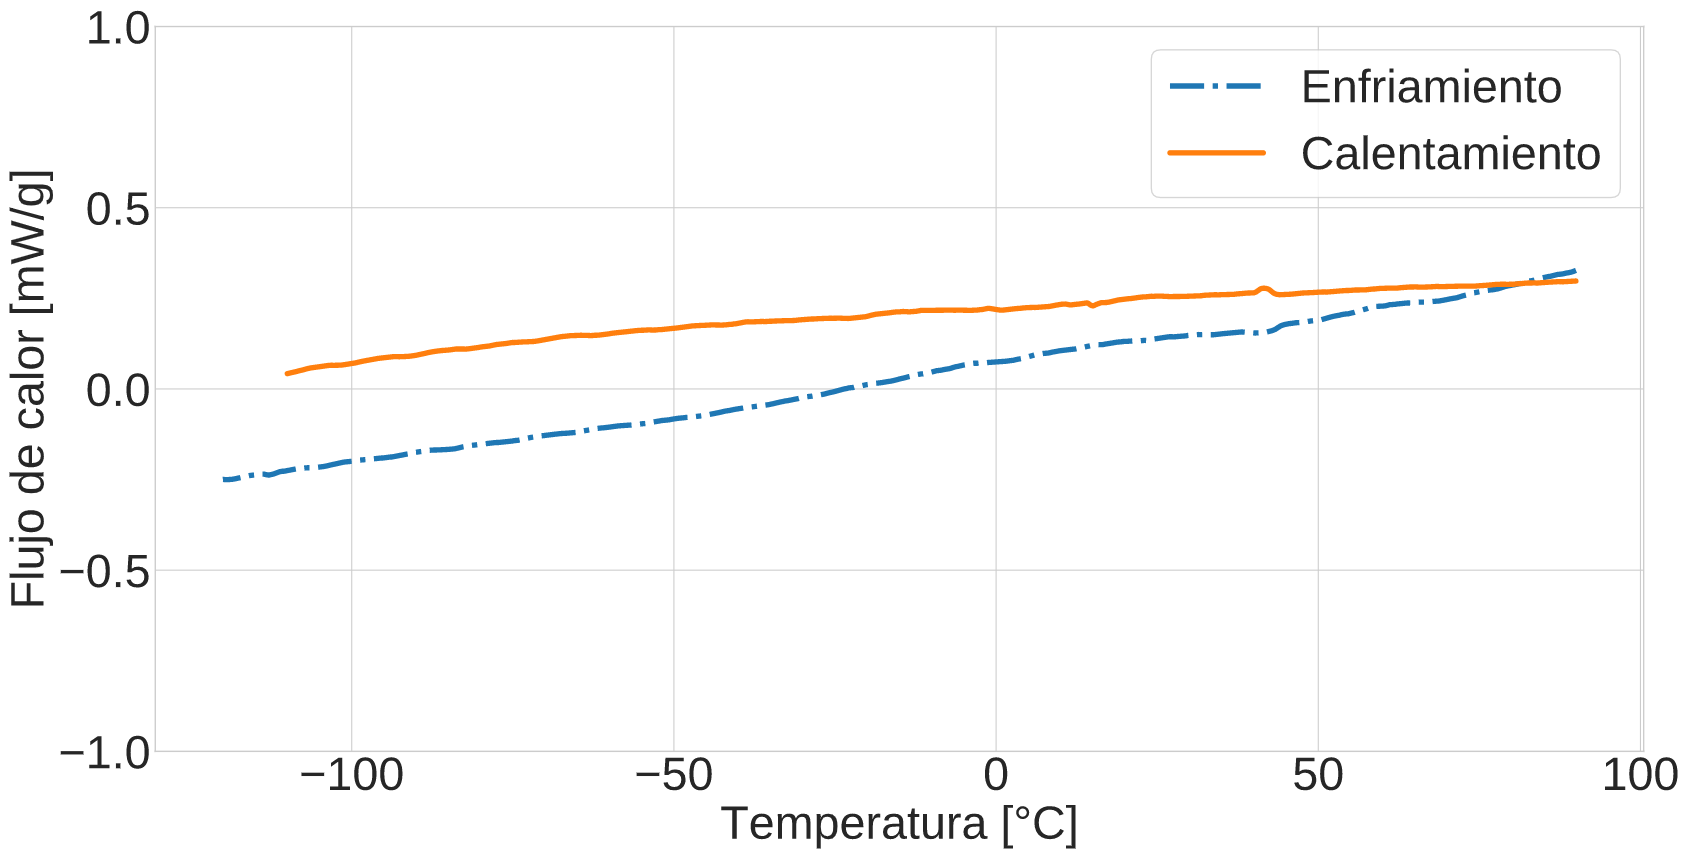
\includegraphics[scale=0.06]{img/DSCNiPoor/500}}\qquad
					\subfloat[Muestra tratada a $600 ^\circ C$]{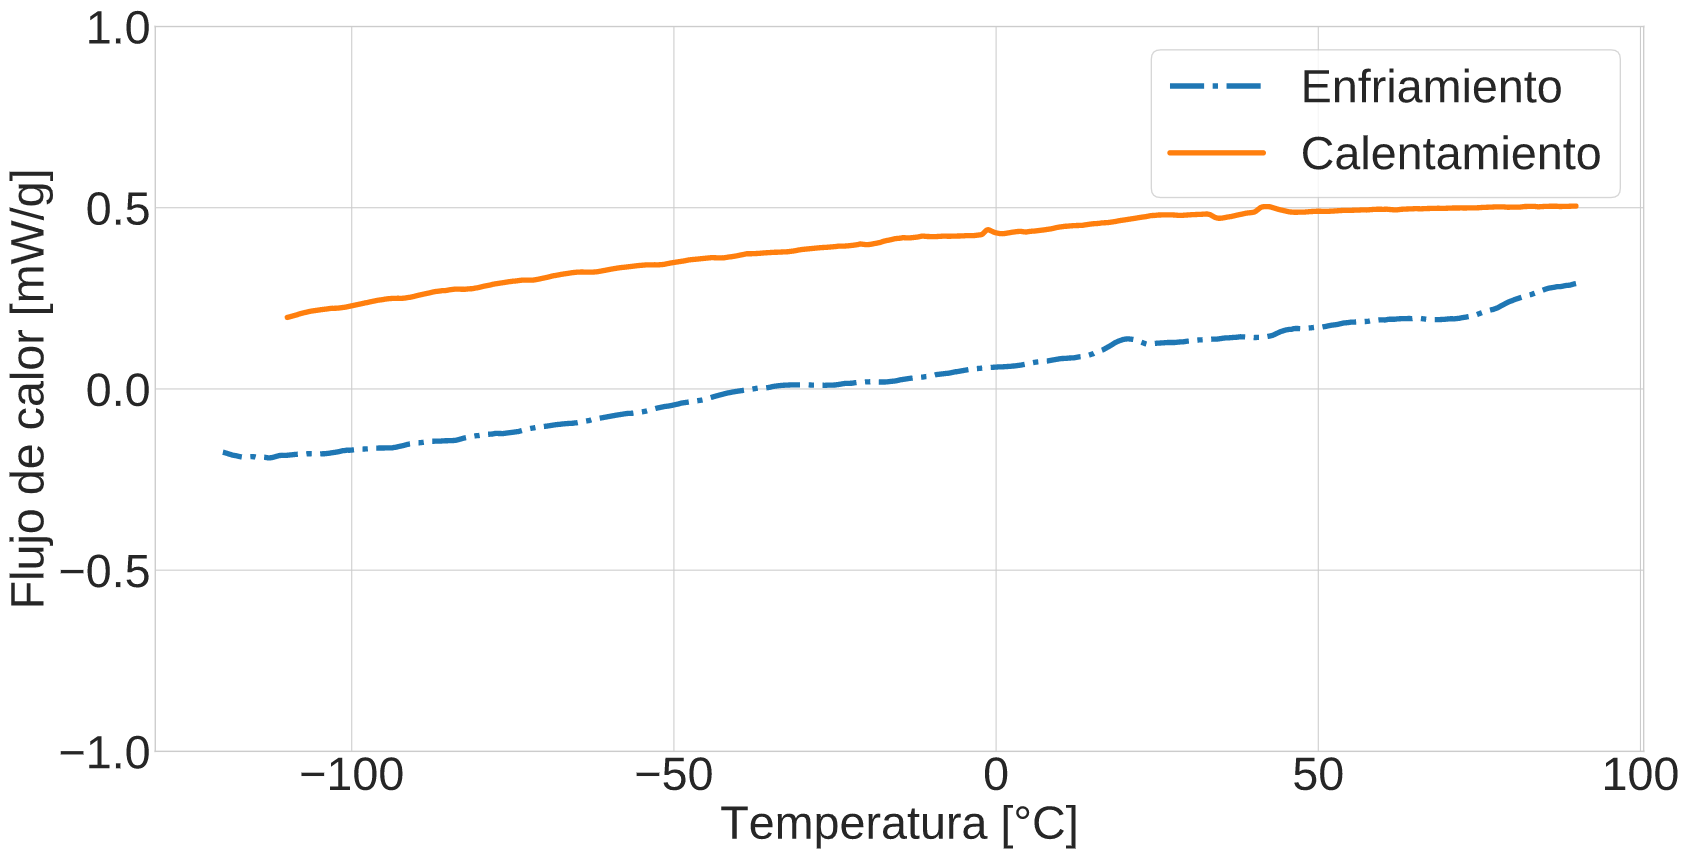
\includegraphics[scale=0.06]{img/DSCNiPoor/600}}} \\
				\noindent\makebox[\linewidth][c]{
					\subfloat[Muestra tratada a $700 ^\circ C$]{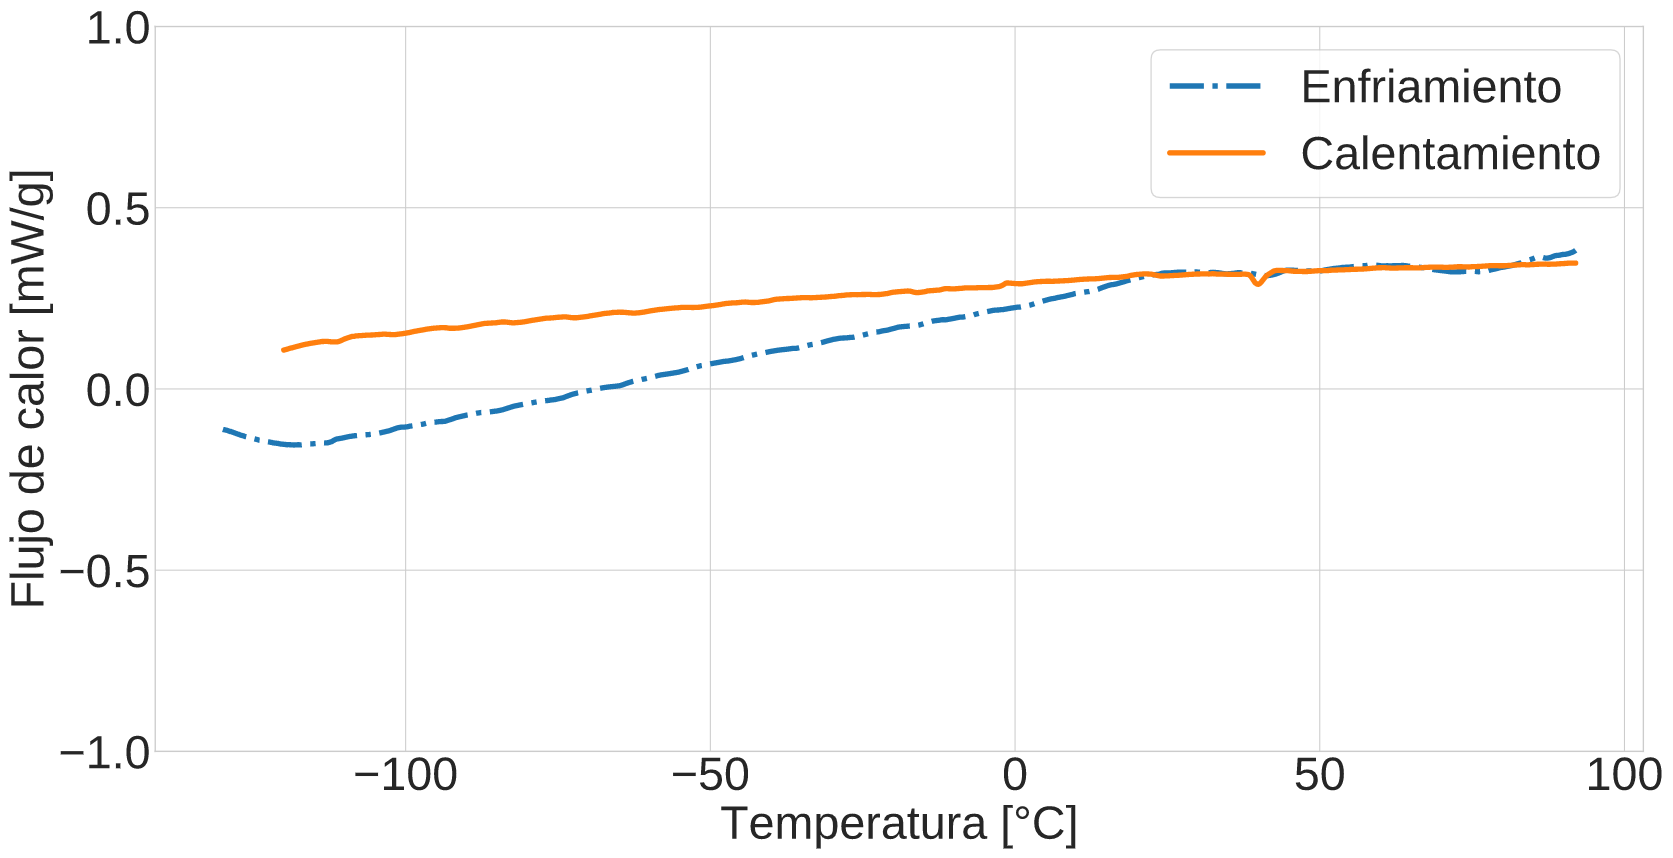
\includegraphics[scale=0.06]{img/DSCNiPoor/700}}\qquad
					\subfloat[Muestra tratada a $800 ^\circ C$]{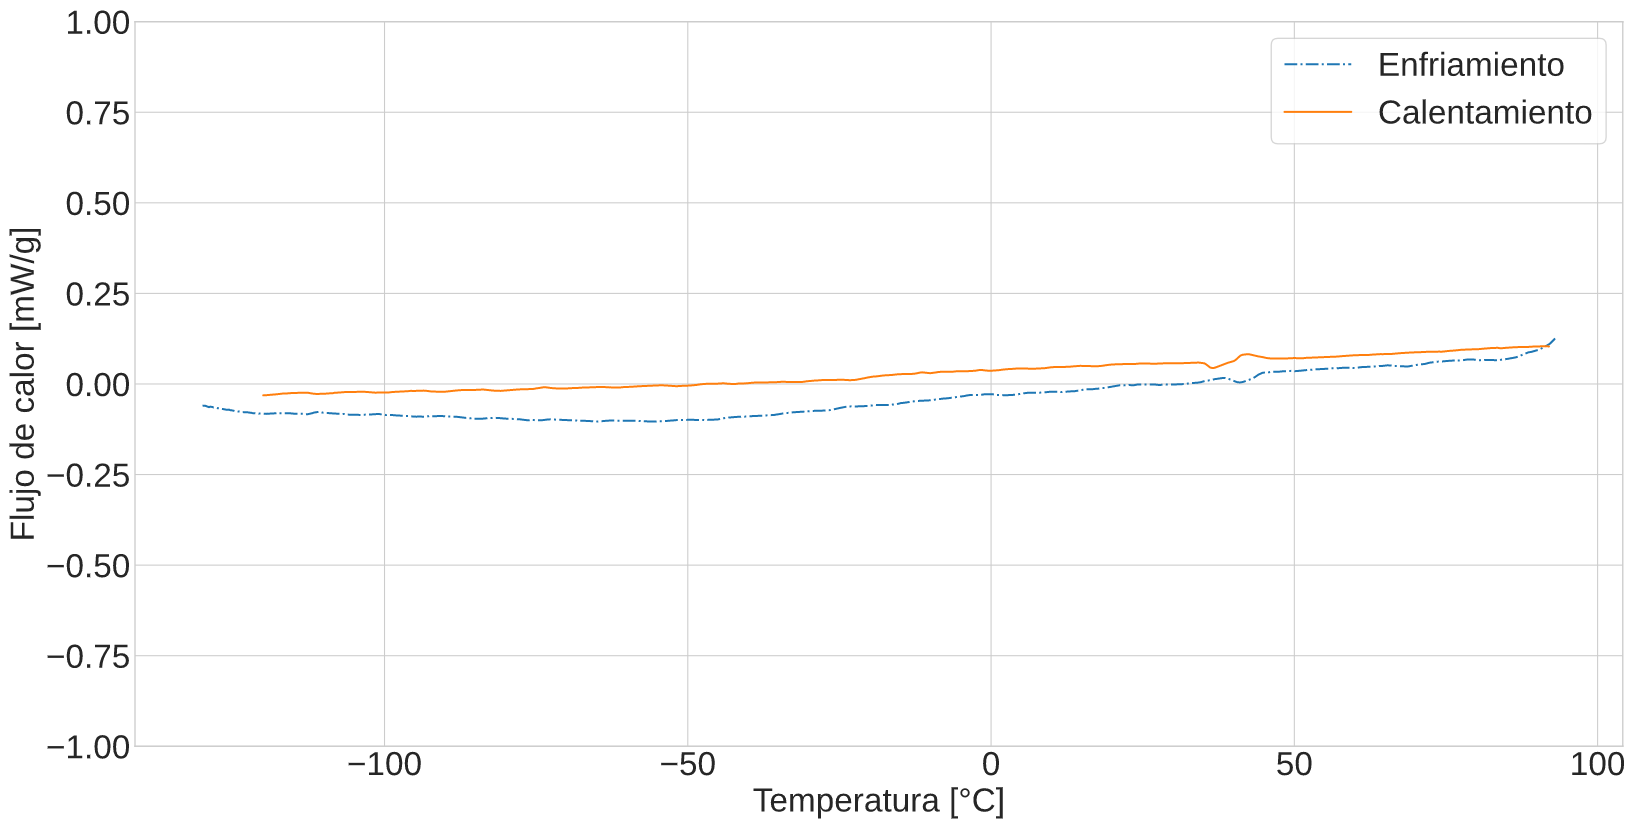
\includegraphics[scale=0.06]{img/DSCNiPoor/800}}}
				\caption*{Curvas de DSC para las distintas muestras.}
			\end{figure}	
		\end{frame}
	\subsection{Ricas en $Ni$}	
		\begin{frame}{Fases obtenidas}
			\begin{figure}[H]
			\captionsetup[subfloat]{labelformat=empty}
				\subfloat[Muestra a $500 ^\circ C$]{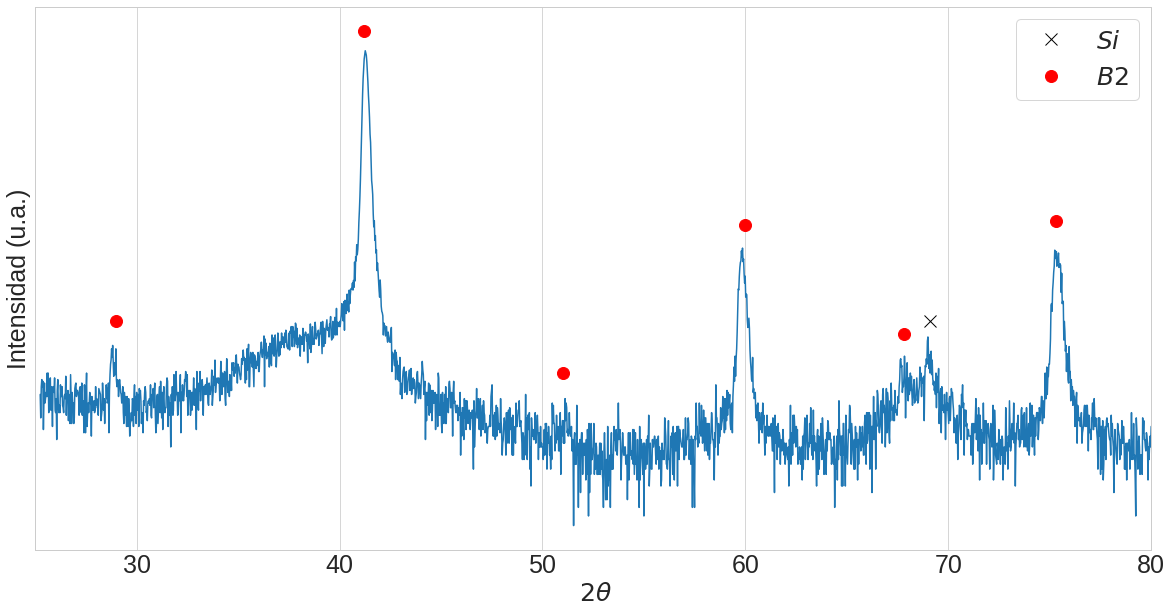
\includegraphics[scale=0.1]{img/RX/NiRich_500.png}} \qquad
				\subfloat[Muestra a $600 ^\circ C$]{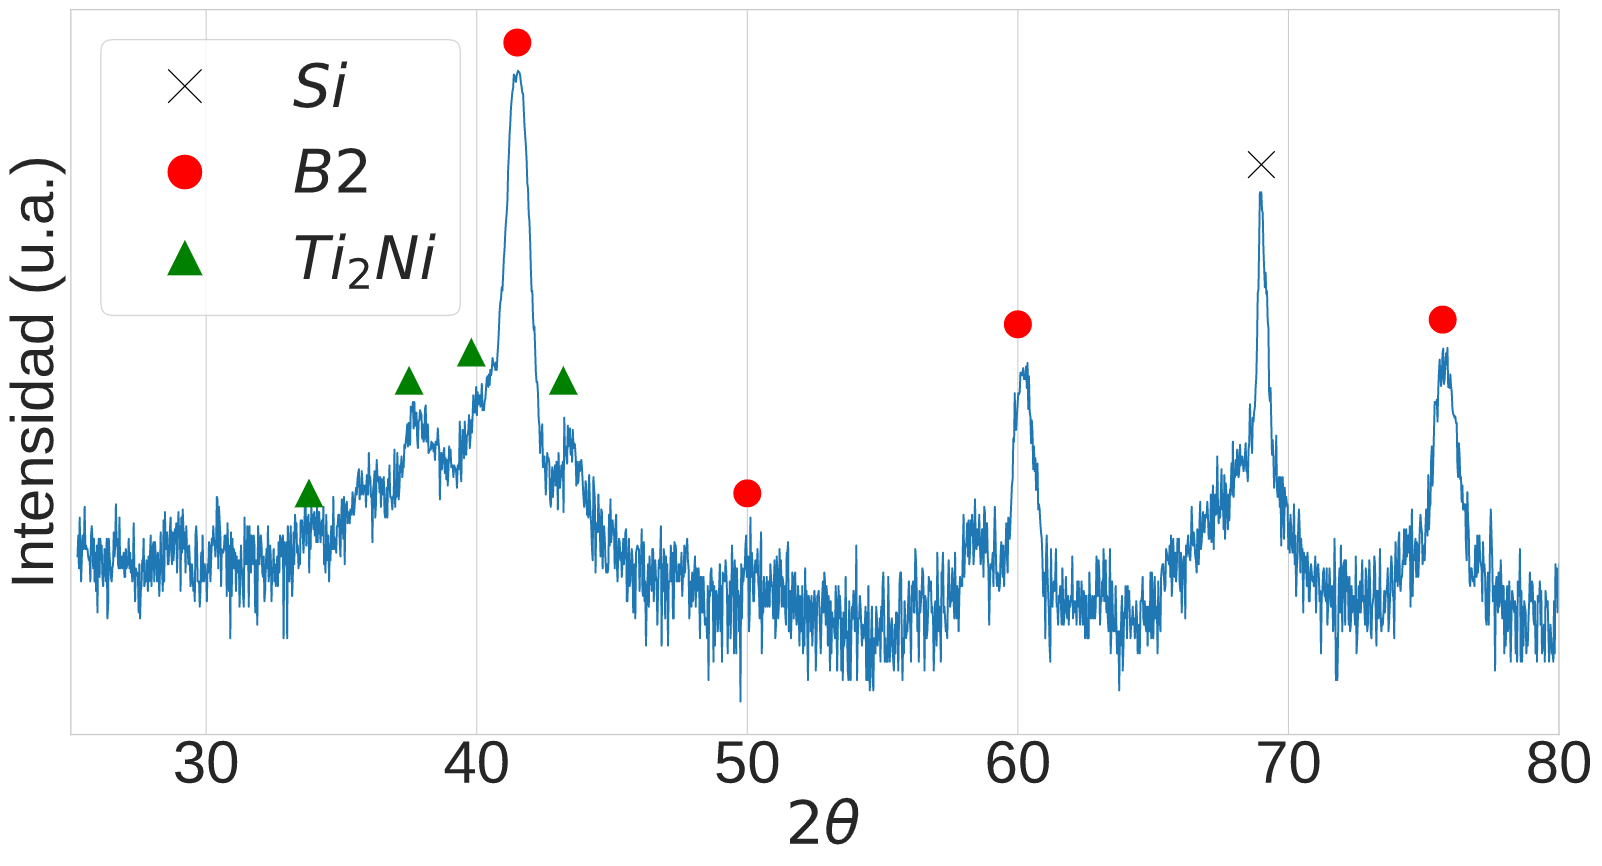
\includegraphics[scale=0.1]{img/RX/NiRich_600.png}} \\
				\subfloat[Muestra a $700 ^\circ C$]{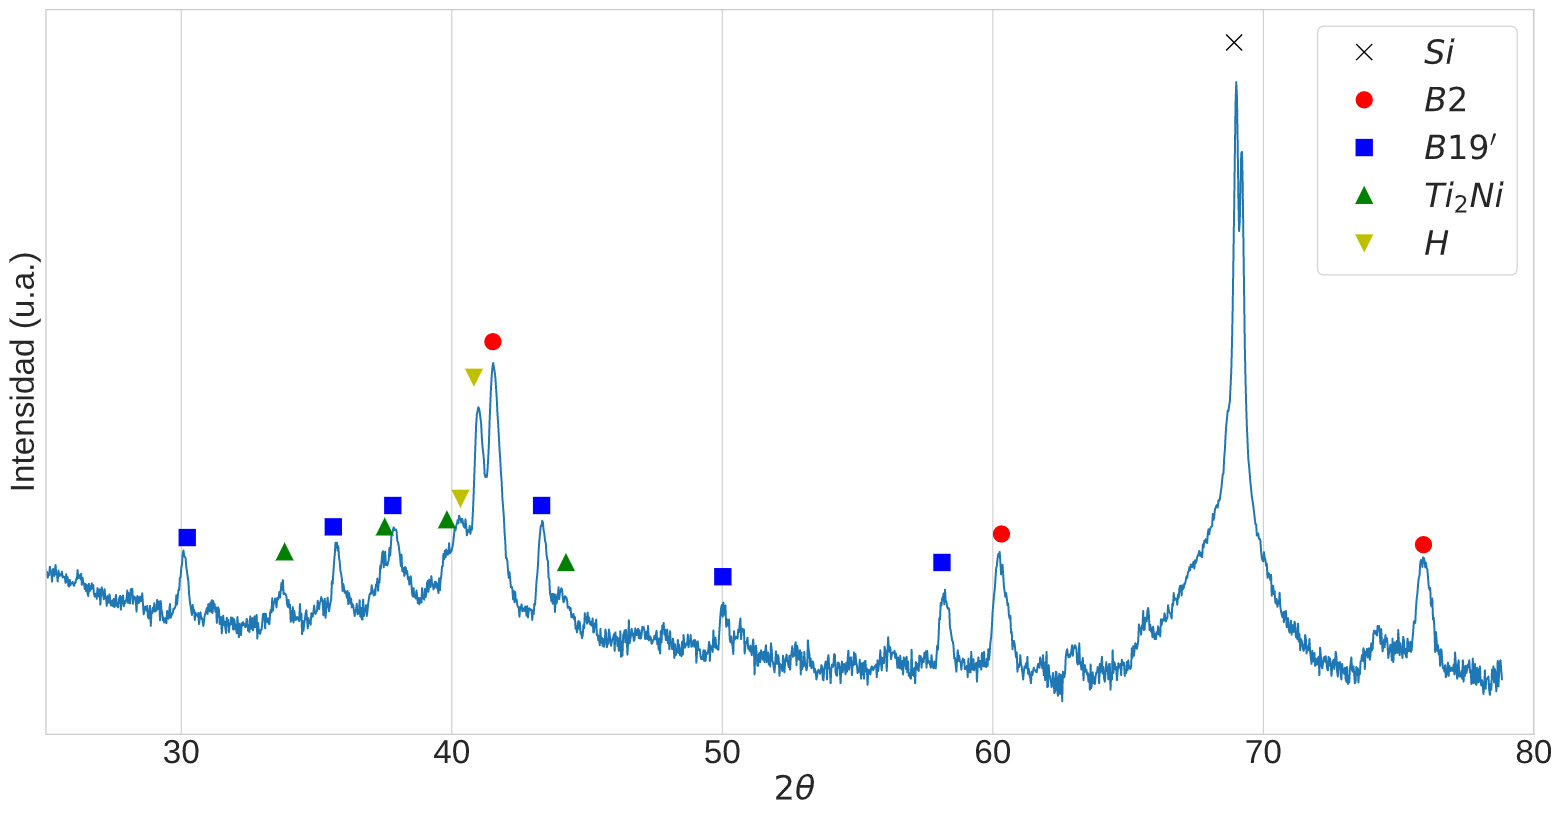
\includegraphics[scale=0.076]{img/RX/NiRich_700.png}} \qquad
				\subfloat[Muestra a $800 ^\circ C$]{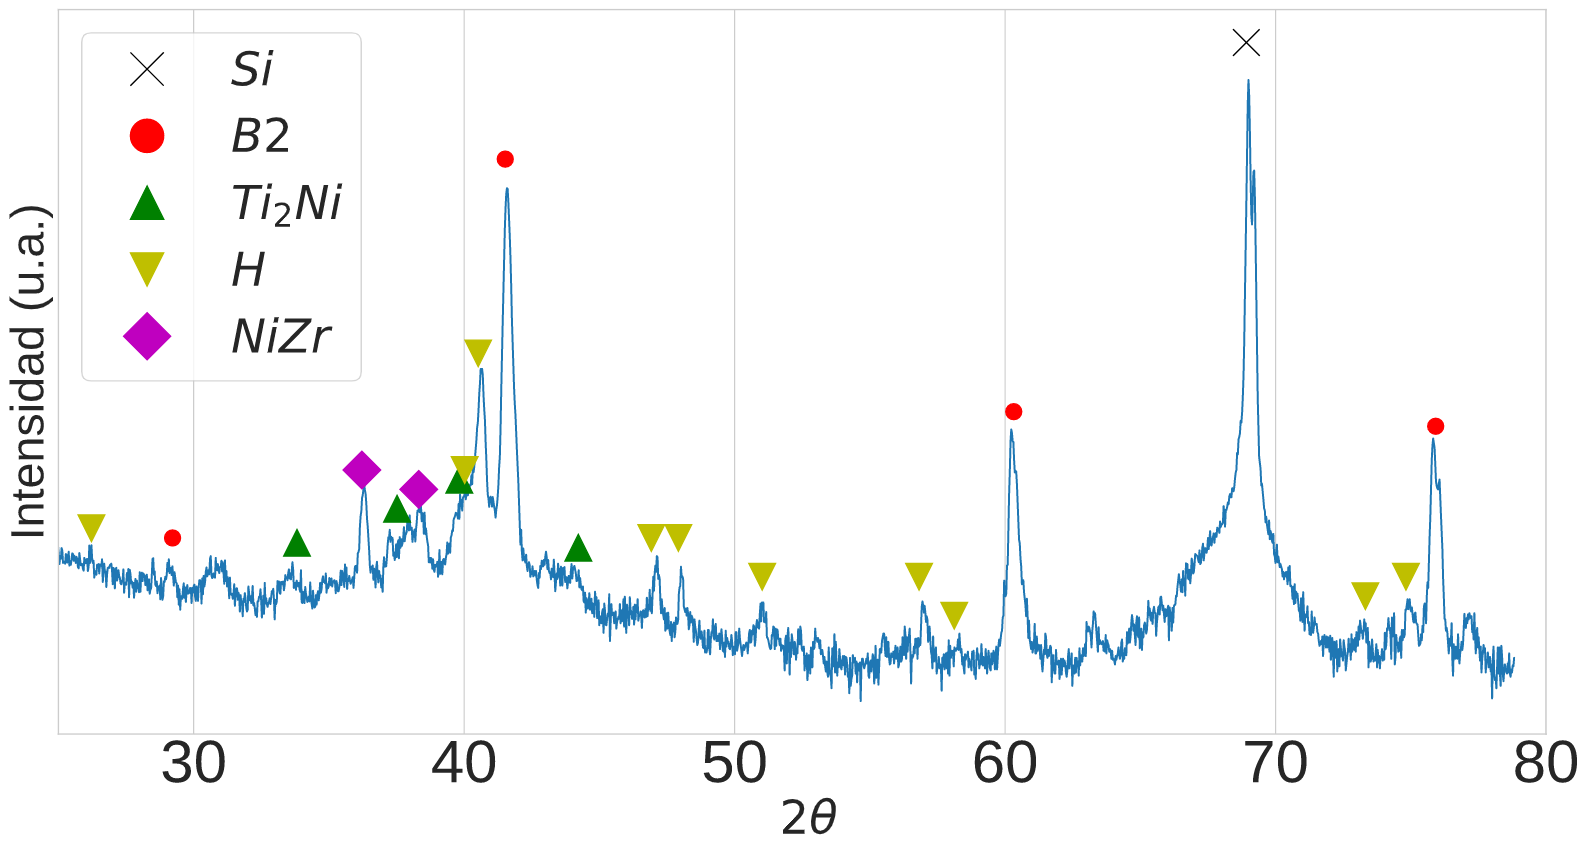
\includegraphics[scale=0.1]{img/RX/NiRich_800.png}} \\
				\caption*{Patrones de difracción para las muestras pobres en $Ni$.}
			\end{figure}		
		\end{frame}

		\begin{frame}{Imágenes obtenidas por TEM}
			 \begin{figure}[H]
			 	\captionsetup[subfloat]{labelformat=empty}
				\centering
				\subfloat[Muestra a $500 ^\circ C$]{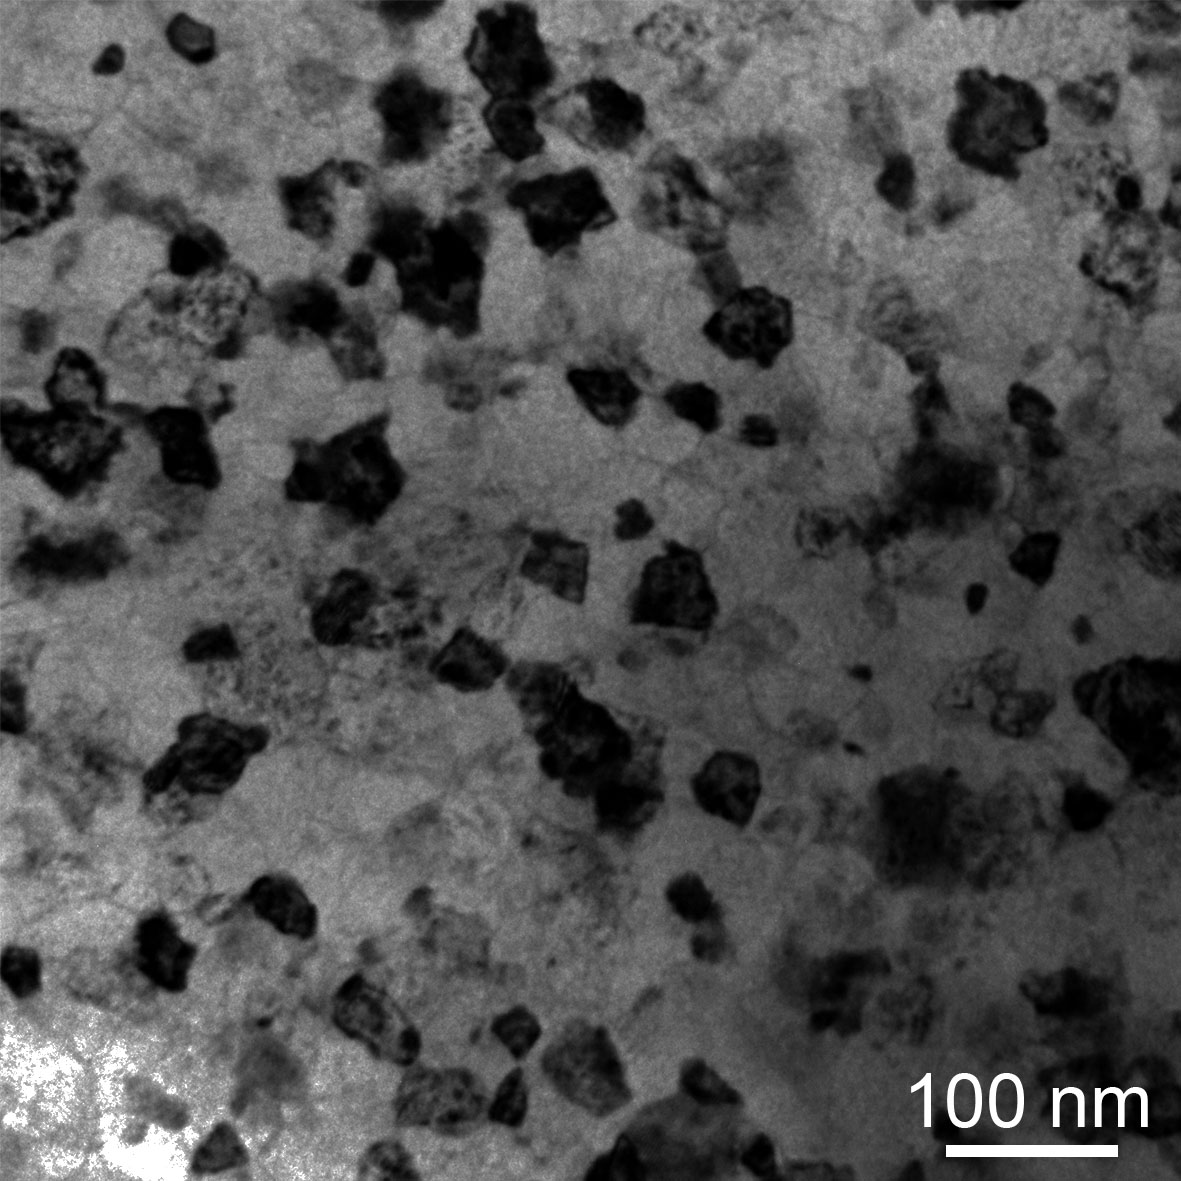
\includegraphics[scale=0.2]{img/TEM/Fig27a.jpg}} \qquad
				\subfloat[Muestra a $600 ^\circ C$]{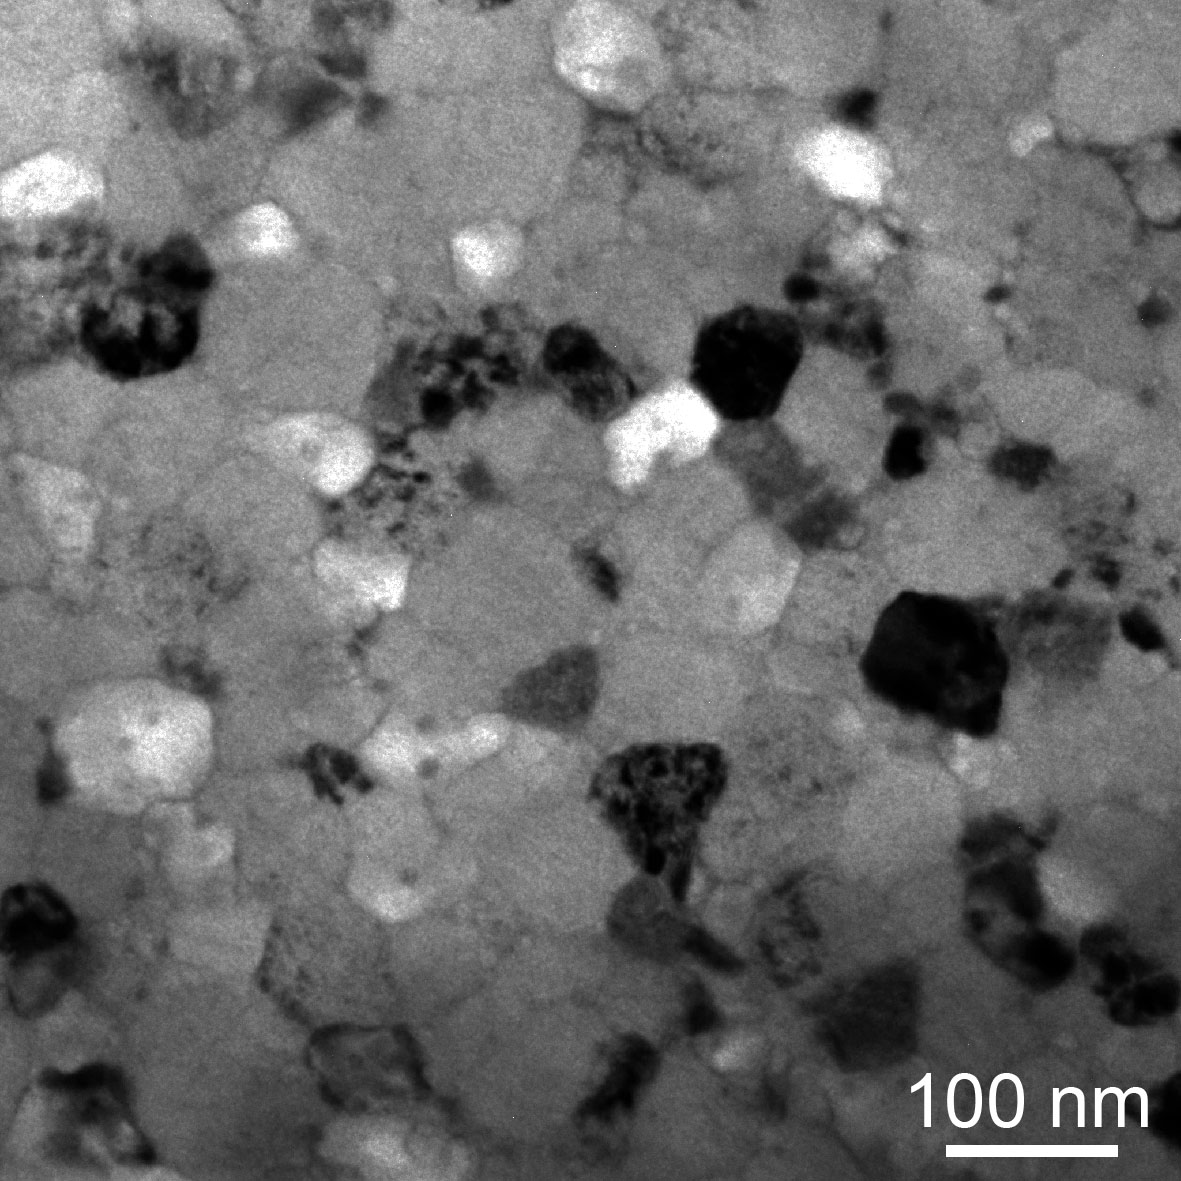
\includegraphics[scale=0.2]{img/TEM/Fig27b.jpg}} \\
				\subfloat[Muestra a $700 ^\circ C$]{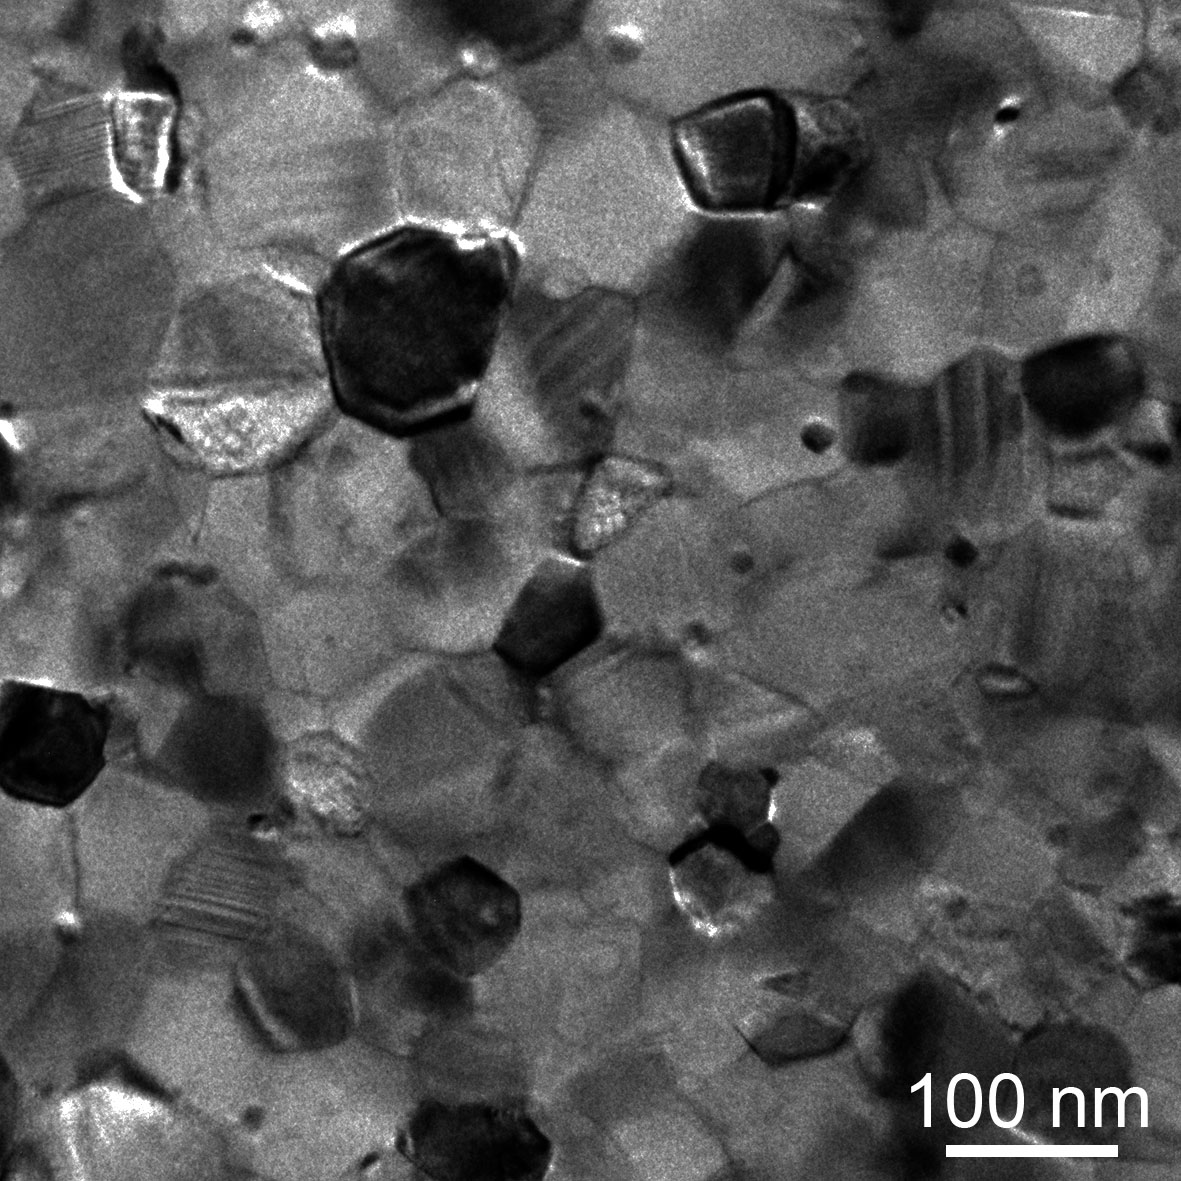
\includegraphics[scale=0.2]{img/TEM/Fig27c.jpg}}	\qquad
				\subfloat[Muestra a $800 ^\circ C$]{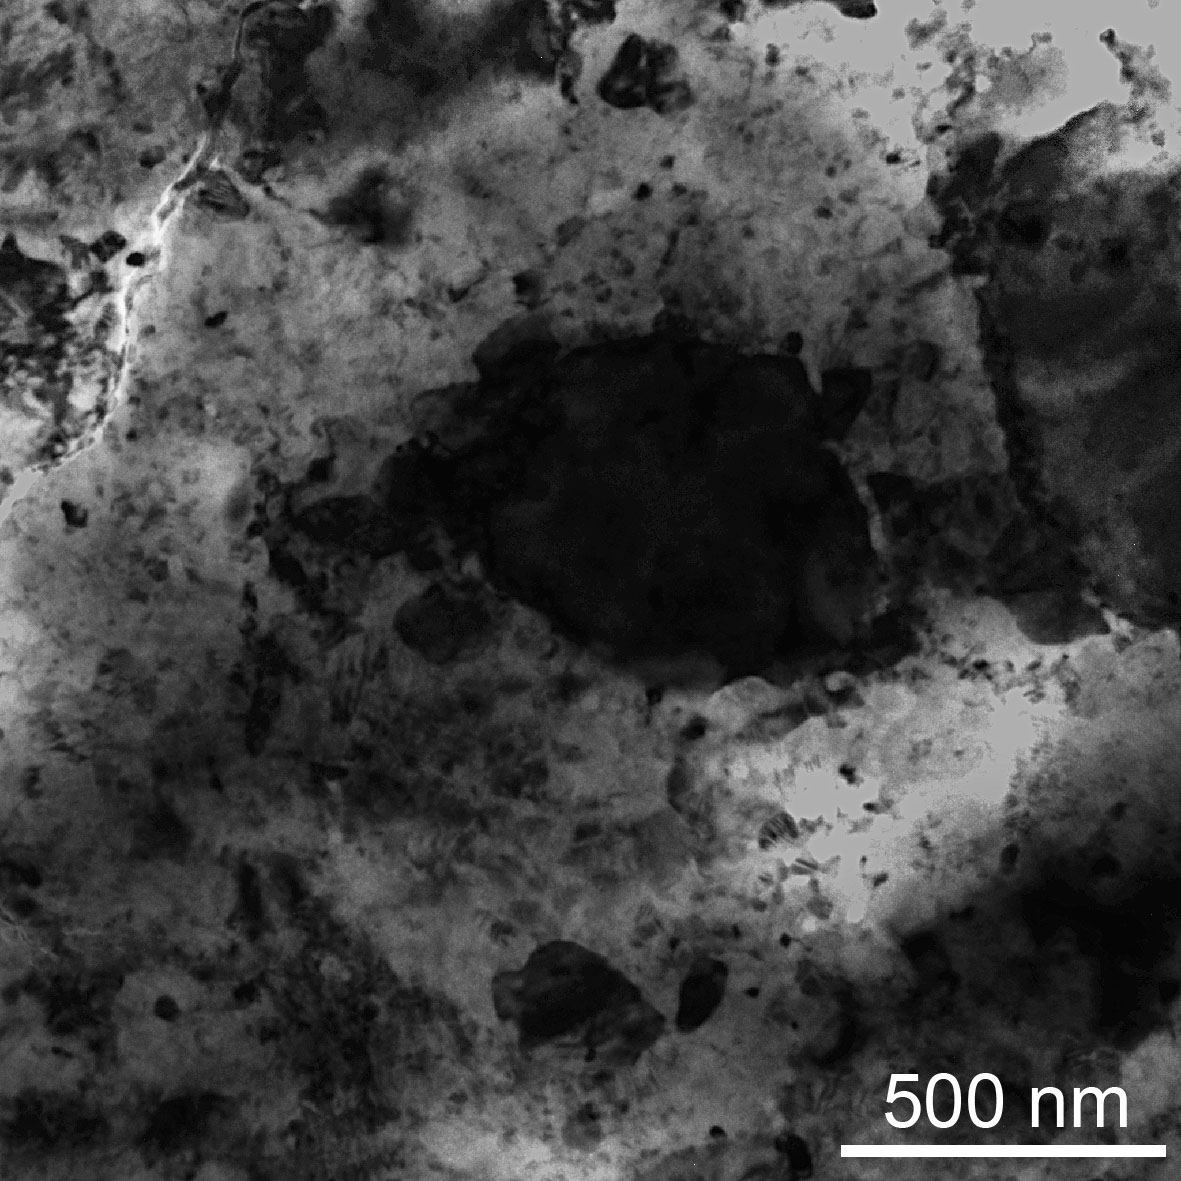
\includegraphics[scale=0.2]{img/TEM/Fig27d.jpg}}
				\caption*{Imágenes de TEM para las muestras ricas en $Ni$.}
				\label{TEMNiRich}
			\end{figure}
		\end{frame}
		
		\begin{frame}
			\begin{figure}[H]
				\captionsetup[subfloat]{labelformat=empty}
				\noindent\makebox[\linewidth][c]{
					\subfloat[Muestra tratada a $500 ^\circ C$]{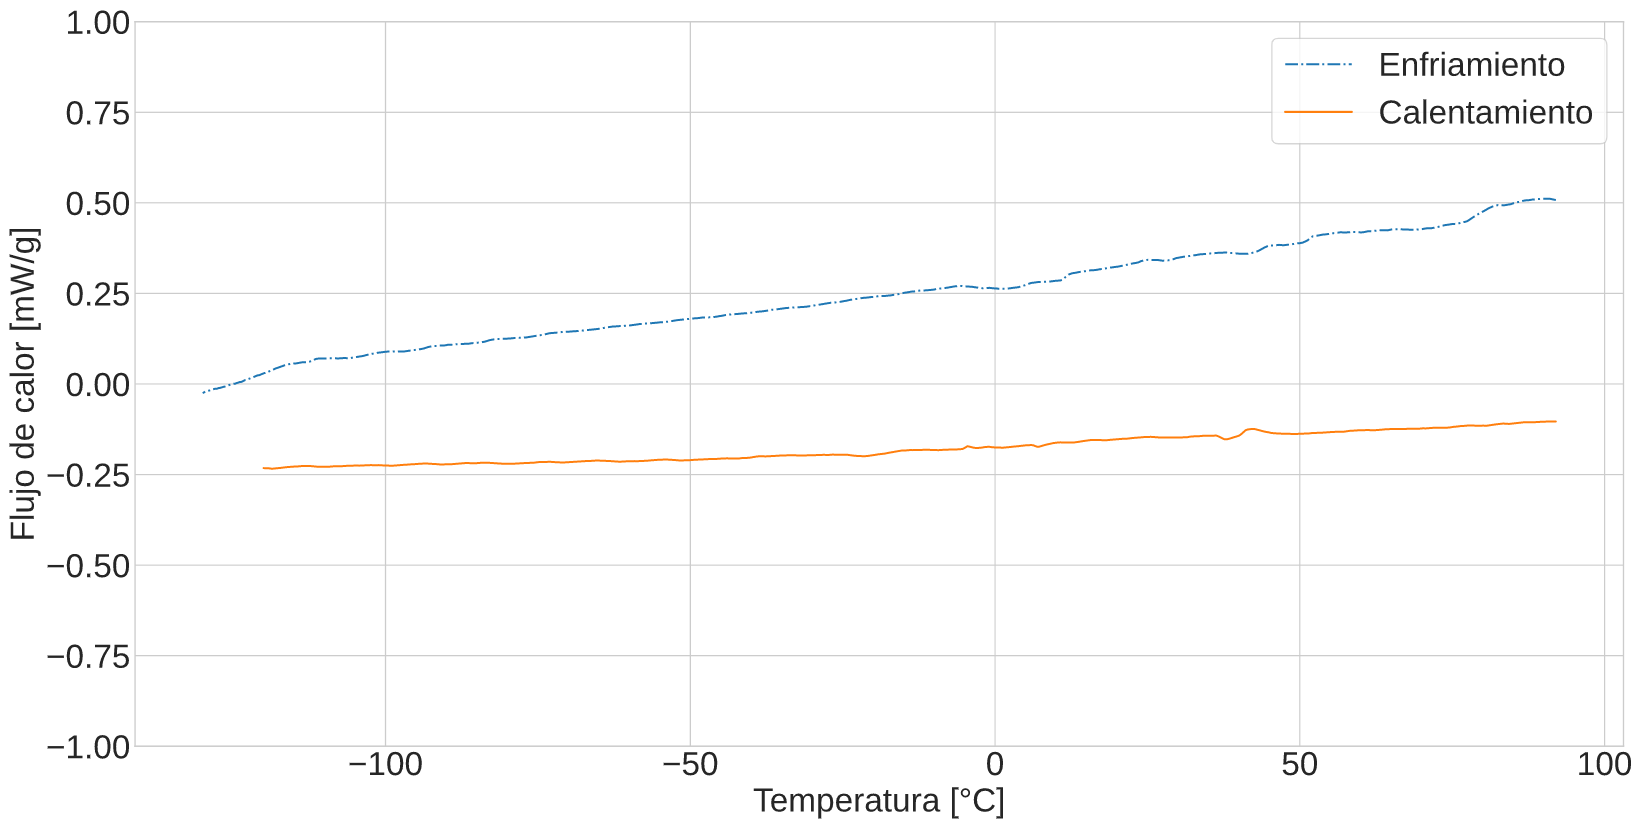
\includegraphics[scale=0.09]{img/DSCNiRich/500NiRich}}
					\subfloat[Muestra tratada a $600 ^\circ C$]{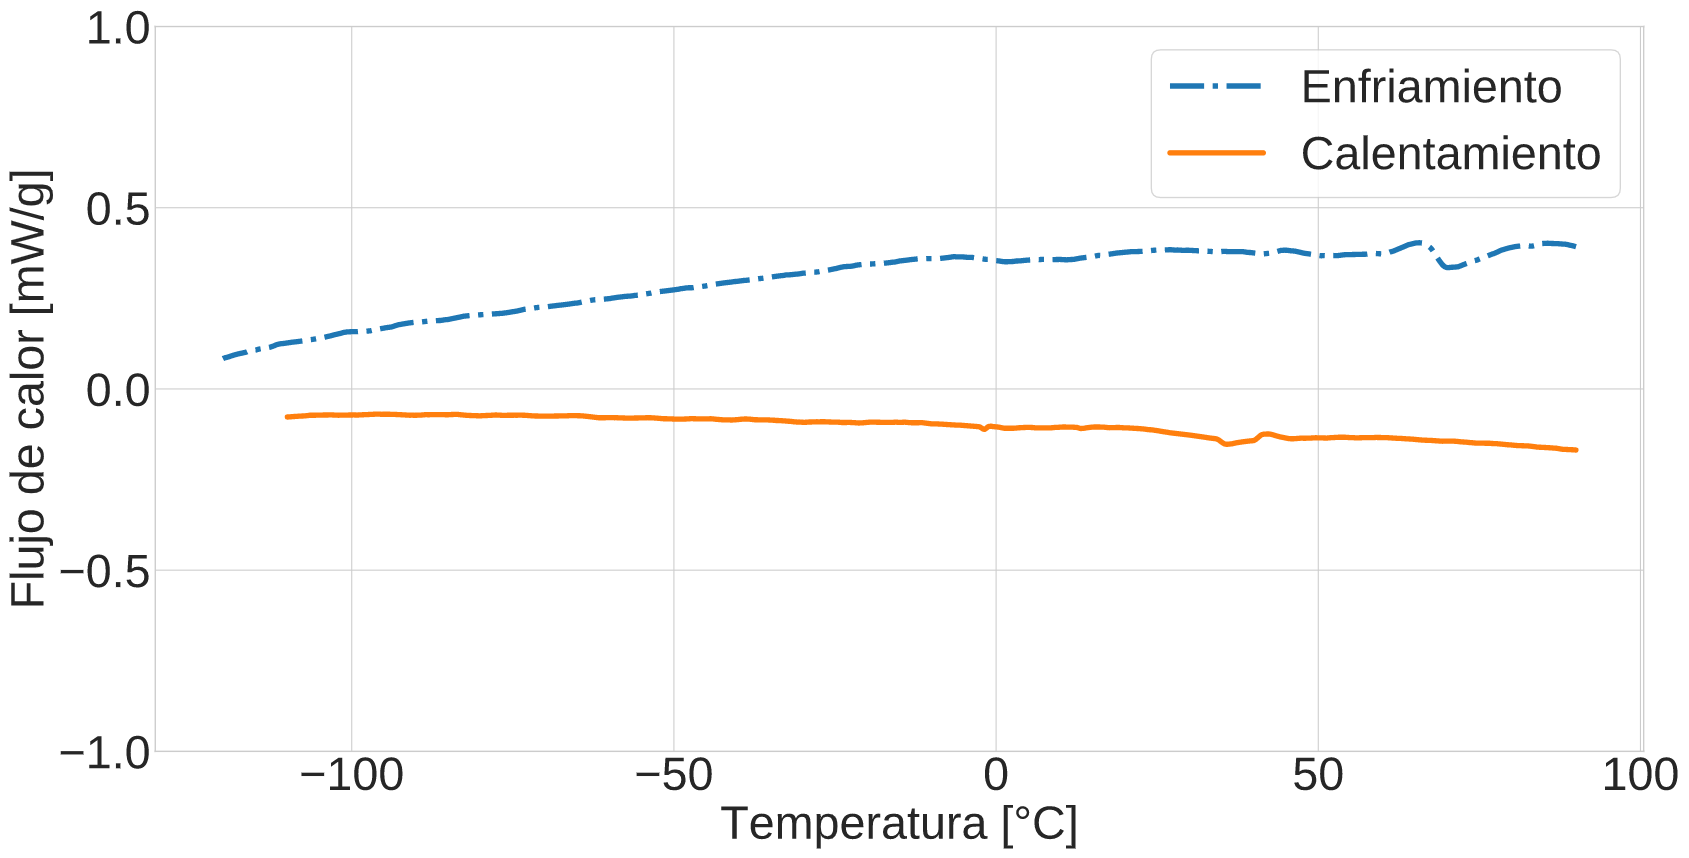
\includegraphics[scale=0.09]{img/DSCNiRich/600NiRich}}}\\
					
				\noindent\makebox[\linewidth][c]{
				\subfloat[Muestra tratada a $700 ^\circ C$]
				{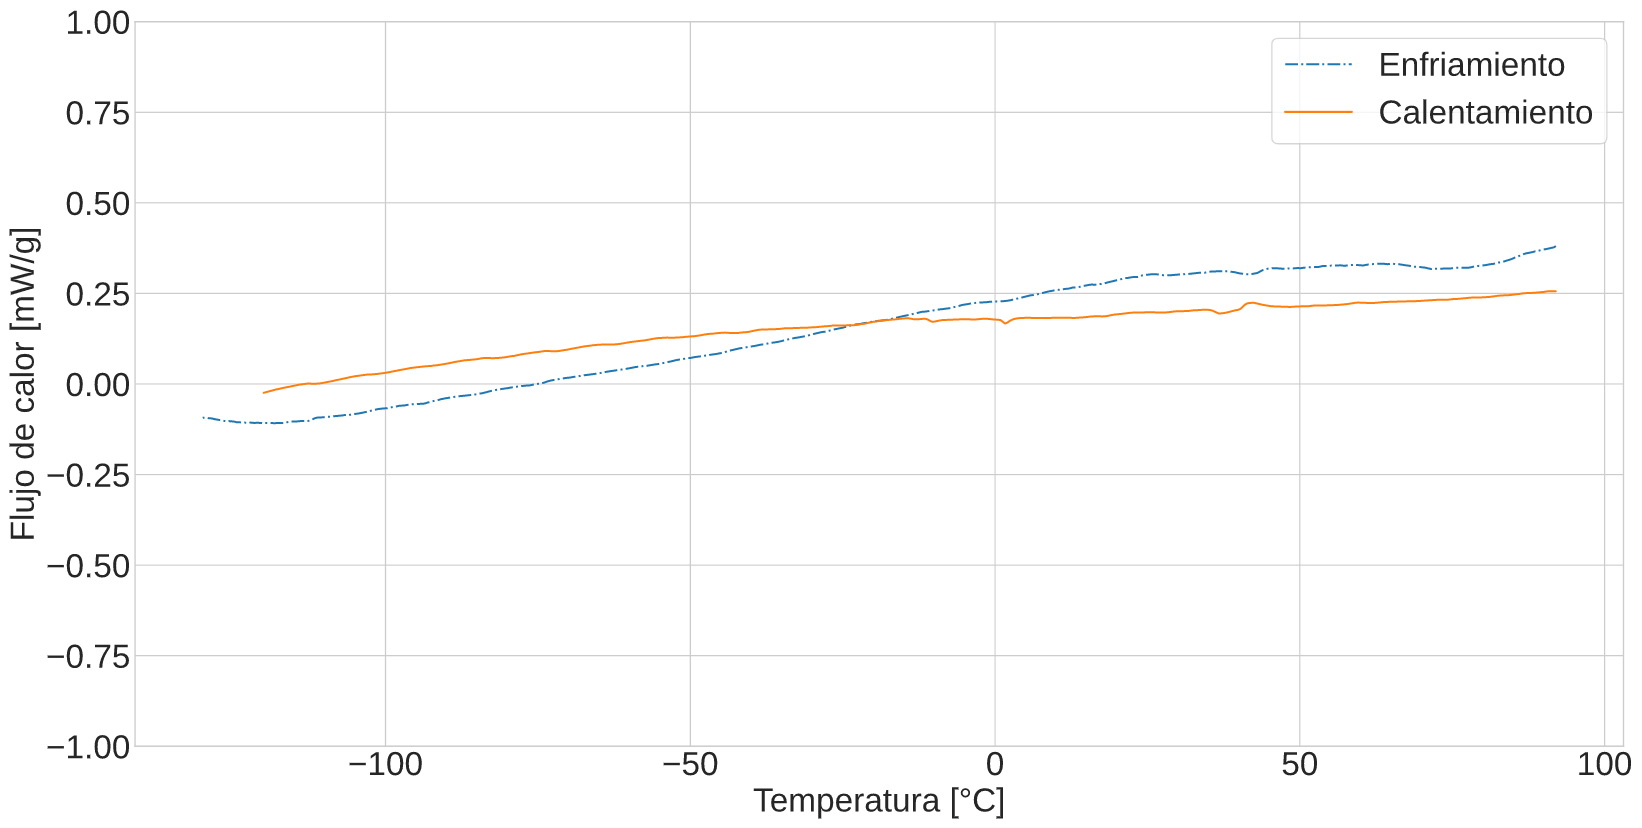
\includegraphics[scale=0.09]{img/DSCNiRich/700NiRich}}}
				 \caption*{Curvas de DSC para muestras ricas en $Ni$ tratadas a diferentes temperaturas.}	
			\end{figure}		
		\end{frame}
		
		\begin{frame}{Curvas de Resistividad}
			\begin{figure}[H]
			\captionsetup[subfloat]{labelformat=empty}
				\centering
				\subfloat[Muestra a $500 ^\circ C$]{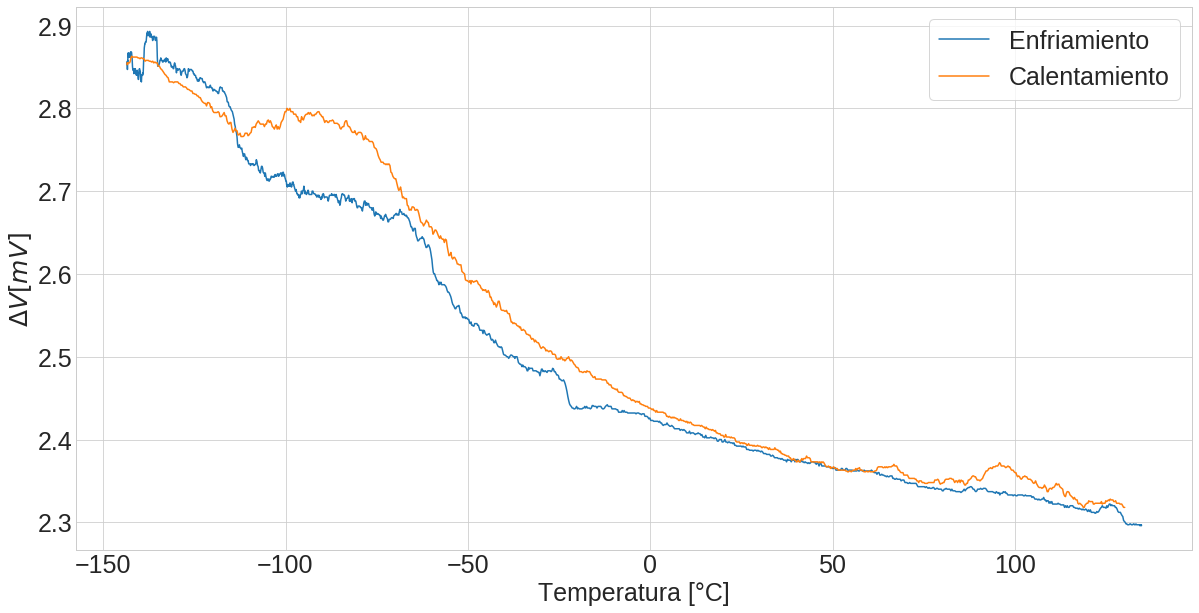
\includegraphics[scale=0.09]{img/Resistance_500.png}} \qquad
				\subfloat[Muestra a $600 ^\circ C$]{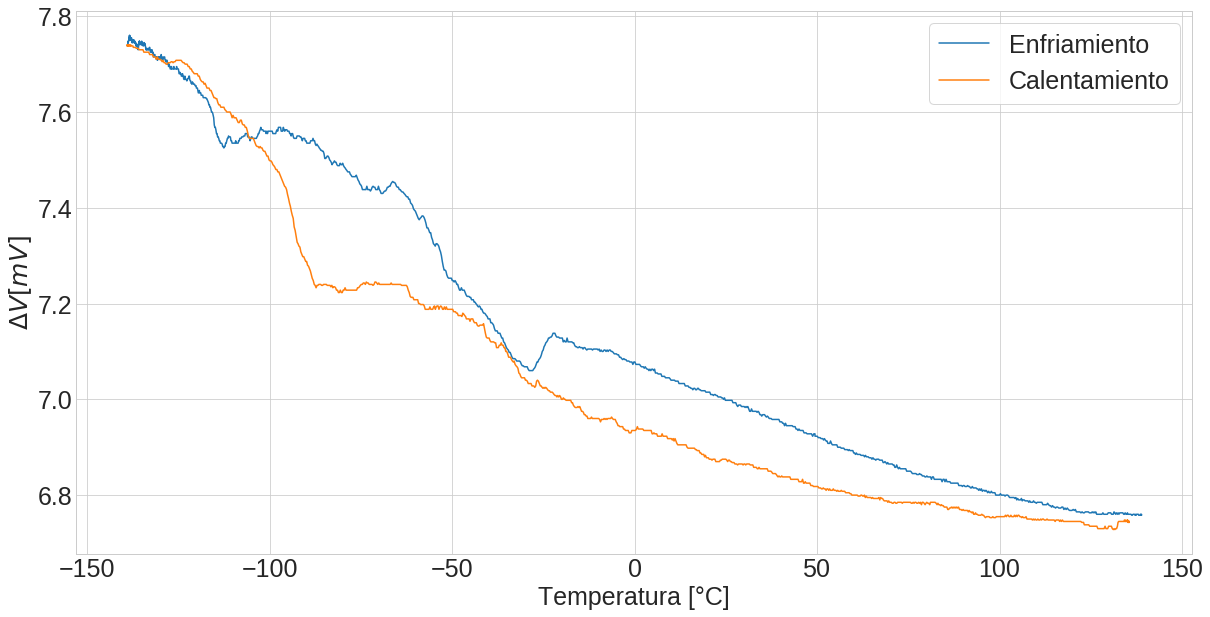
\includegraphics[scale=0.09]{img/Resistance_600.png}}\\
				\subfloat[Muestra a $800 ^\circ C$]{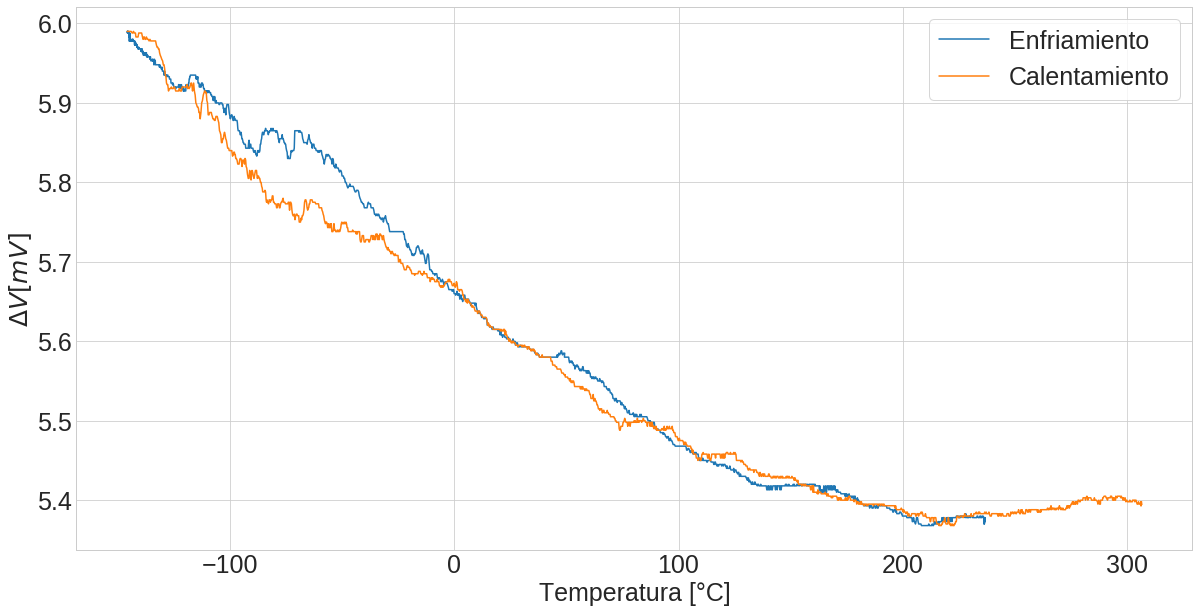
\includegraphics[scale=0.09]{img/Resistance_800.png}} 
				\caption*{Curvas medidas por el método de resistividad de cuatro puntas en las cuales no fue posible hallar en forma precisa las temperatura de transformación.}
				\label{Failures}
			\end{figure}
		\end{frame}
		
		\begin{frame}
			\begin{figure}[H]
				\centering
				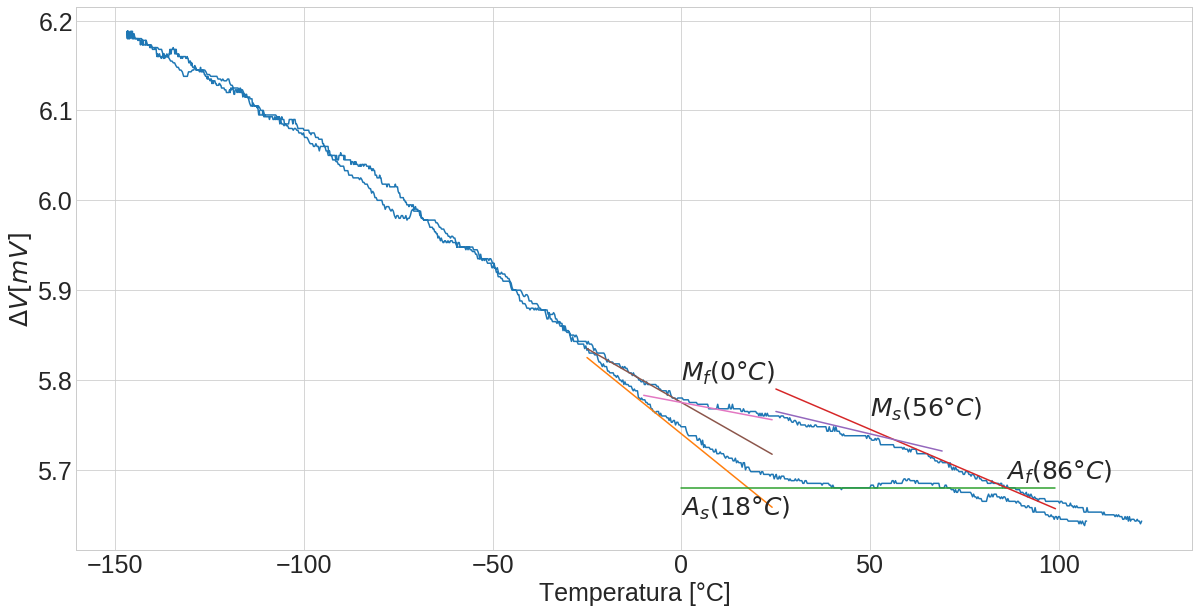
\includegraphics[scale=0.2]{img/Resistance_700.png}
				\caption*{Curva medida por el método de resistividad de cuatro puntas para la muestra tratada a 700$^\circ C$.}
				\label{Failures}
			\end{figure}
		\end{frame}
	

\section{Conclusión}

\end{document}
%		\begin{frame}{Difracción por RX}
%		\begin{columns}
%		\begin{column}{.49\textwidth}
%		\end{column}
%		\begin{column}{.49\textwidth}
%		\end{column}
%		\end{columns}
